\documentclass[a4paper,11pt]{book}
\usepackage{listings}
\usepackage[utf8]{inputenc}
\usepackage[spanish]{babel}
\usepackage{amsmath}
\usepackage{amssymb}
\usepackage{amsthm}
\usepackage{xspace}

\decimalpoint
\usepackage{dcolumn}
\newcolumntype{.}{D{.}{\esperiod}{-1}}
\makeatletter
\addto\shorthandsspanish{\let\esperiod\es@period@code}
\makeatother

\RequirePackage{verbatim}
\usepackage{fancyhdr}
\usepackage{graphicx}
\usepackage{float}
\usepackage{afterpage}
\usepackage{longtable}
\usepackage[pdfborder={000}]{hyperref}

\newcommand{\myTitle}{Análisis de seguridad y optimización de generadores pseudoaleatorios basados en LFSR\xspace}
\newcommand{\myDegree}{Grado en Ingeniería Informática\xspace}
\newcommand{\myName}{Joaquín Sergio García Ibáñez\xspace}
\newcommand{\myProf}{Jesús García Miranda\xspace}
\newcommand{\myFaculty}{Escuela Técnica Superior de Ingenierías Informática y de Telecomunicación\xspace}
\newcommand{\myFacultyShort}{E.T.S. de Ingenierías Informática y de Telecomunicación\xspace}
\newcommand{\myDepartment}{Departamento de Álgebra\xspace}
\newcommand{\myUni}{\protect{Universidad de Granada}\xspace}
\newcommand{\myLocation}{Granada\xspace}
\newcommand{\myTime}{\today\xspace}

\hypersetup{
pdfauthor = {\myName},
pdftitle = {\myTitle},
pdfsubject = {Criptografía, LFSR, generadores pseudoaleatorios},
pdfkeywords = {LFSR, Berlekamp-Massey, complejidad lineal, generadores de flujo, criptografía},
pdfcreator = {LaTeX},
pdfproducer = {pdflatex}
}

\usepackage{url}
\usepackage{colortbl,longtable}
\usepackage[stable]{footmisc}

\setlength{\headheight}{15pt}
\pagestyle{fancy}
\fancyhf{}
\fancyhead[LO]{\leftmark}
\fancyhead[RE]{\rightmark}
\fancyhead[RO,LE]{\textbf{\thepage}}
\renewcommand{\chaptermark}[1]{\markboth{\textbf{#1}}{}}
\renewcommand{\sectionmark}[1]{\markright{\textbf{\thesection. #1}}}

\fancypagestyle{plain}{
  \fancyhf{}
  \fancyfoot[C]{\thepage}
  \renewcommand{\headrulewidth}{0pt}
  \renewcommand{\footrulewidth}{0pt}
}

\newcommand{\HRule}{\rule{\linewidth}{0.5mm}}

\newtheorem{definicion}{Definición}[chapter]
\newtheorem{ejemplo}{Ejemplo}[chapter]
\newtheorem{proposicion}{Proposición}[chapter]

\definecolor{gray97}{gray}{.97}
\definecolor{gray75}{gray}{.75}
\definecolor{gray45}{gray}{.45}
\definecolor{gray30}{gray}{.94}

\lstset{
  frame=Ltb,
  framerule=0.5pt,
  aboveskip=0.5cm,
  framextopmargin=3pt,
  framexbottommargin=3pt,
  framexleftmargin=0.1cm,
  framesep=0pt,
  rulesep=.4pt,
  backgroundcolor=\color{gray97},
  rulesepcolor=\color{black},
  stringstyle=\ttfamily,
  showstringspaces=false,
  basicstyle=\scriptsize\ttfamily,
  commentstyle=\color{gray45},
  keywordstyle=\bfseries,
  numbers=left,
  numbersep=6pt,
  numberstyle=\tiny,
  numberfirstline=false,
  breaklines=true,
}

\lstdefinestyle{Python}{
  basicstyle=\small\ttfamily,
  frame=single,
  language=Python,
  numbers=left,
  backgroundcolor=\color{gray97},
}

\definecolor{termbg}{rgb}{0.13,0.13,0.13}
\definecolor{termfg}{rgb}{0.92,0.92,0.92}
\definecolor{termgreen}{rgb}{0.65,0.85,0.45}

\lstdefinestyle{Terminal}{
  basicstyle=\small\ttfamily\color{termfg},
  backgroundcolor=\color{termbg},
  frame=single,
  framesep=6pt,
  numbers=none,
  showspaces=false,
  showstringspaces=false,
  breaklines=true,
  literate={→}{{\textcolor{termgreen}{$\rightarrow$}}}1
           {✓}{{\textcolor{termgreen}{\checkmark}}}1
           {✗}{{\textcolor{red}{$\times$}}}1
           {á}{{\'a}}1 {é}{{\'e}}1 {í}{{\'\i}}1 {ó}{{\'o}}1 {ú}{{\'u}}1 {ñ}{{\~n}}1
           {Á}{{\'A}}1 {É}{{\'E}}1 {Í}{{\'I}}1 {Ó}{{\'O}}1 {Ú}{{\'U}}1 {Ñ}{{\~N}}1,
}

\makeatletter
\def\clearpage{%
  \ifvmode
    \ifnum \@dbltopnum =\m@ne
      \ifdim \pagetotal <\topskip
        \hbox{}
      \fi
    \fi
  \fi
  \newpage
  \thispagestyle{empty}
  \write\m@ne{}
  \vbox{}
  \penalty -\@Mi
}
\makeatother

\usepackage{pdfpages}
\usepackage{tikz}
\usetikzlibrary{babel}

\begin{document}

\begin{titlepage}

\newlength{\centeroffset}
\setlength{\centeroffset}{-0.5\oddsidemargin}
\addtolength{\centeroffset}{0.5\evensidemargin}
\thispagestyle{empty}

\noindent\hspace*{\centeroffset}\begin{minipage}{\textwidth}

\centering

\includegraphics[width=0.9\textwidth]{images/logo_ugr.jpg}\\[1.4cm]

\textsc{\Large TRABAJO FIN DE GRADO\\[0.2cm]}
\textsc{GRADO EN INGENIERÍA INFORMÁTICA}\\[1cm]

{\Huge\bfseries Análisis de seguridad y optimización de\\
generadores pseudoaleatorios basados en LFSR\\}
\noindent\rule[-1ex]{\textwidth}{3pt}\\[3.5ex]

\end{minipage}

\vspace{2.5cm}
\noindent\hspace*{\centeroffset}\begin{minipage}{\textwidth}
\centering

\textbf{Autor}\\ {Joaquín Sergio García Ibáñez}\\[2.5ex]
\textbf{Director}\\
{Jesús García Miranda}\\[2cm]

\includegraphics[width=0.3\textwidth]{images/etsiit_logo.png}\\[0.1cm]
\textsc{Escuela Técnica Superior de Ingenierías Informática y de Telecomunicación}\\
\textsc{---}\\
Granada, abril de 2026
\end{minipage}

\end{titlepage}

\chapter*{}
\thispagestyle{empty}

\cleardoublepage
\thispagestyle{empty}

\begin{center}
{\large\bfseries Análisis de seguridad y optimización de generadores pseudoaleatorios basados en LFSR}\\
\end{center}
\begin{center}
Joaquín Sergio García Ibáñez\\
\end{center}

\noindent{\textbf{Palabras clave}: LFSR, Berlekamp-Massey, complejidad lineal, generadores de flujo, criptografía simétrica, tests NIST}\\

\vspace{0.7cm}
\noindent{\textbf{Resumen}}\\

Los registros de desplazamiento con retroalimentación lineal (LFSR) son la base de muchos
generadores de secuencias cifrantes usados en criptografía de flujo. Por sí solos presentan
vulnerabilidades graves, en particular frente al algoritmo de Berlekamp-Massey, que permite
reconstruir el registro completo a partir de un número pequeño de bits observados. Este trabajo
analiza cuatro generadores basados en LFSR ---Geffe, Shrinking, Self-Shrinking y Alternating
Step--- comparando su complejidad lineal y su comportamiento frente a los tests estadísticos
NIST SP 800-22. El objetivo es identificar cuáles ofrecen mejores garantías de seguridad y
entender por qué.

\cleardoublepage

\thispagestyle{empty}

\begin{center}
{\large\bfseries Security analysis and optimization of LFSR-based pseudorandom generators}\\
\end{center}
\begin{center}
Joaquín Sergio García Ibáñez\\
\end{center}

\noindent{\textbf{Keywords}: LFSR, Berlekamp-Massey, linear complexity, stream ciphers, symmetric cryptography, NIST tests}\\

\vspace{0.7cm}
\noindent{\textbf{Abstract}}\\

Linear Feedback Shift Registers (LFSRs) are the building block of many keystream generators
used in stream ciphers. On their own they have serious weaknesses, most notably against the
Berlekamp-Massey algorithm, which can reconstruct the register from a short observed sequence.
This thesis analyses four LFSR-based generators ---Geffe, Shrinking, Self-Shrinking and
Alternating Step--- comparing their linear complexity and statistical behaviour using the NIST
SP 800-22 test suite. The goal is to identify which ones provide stronger security guarantees
and to understand the reasons behind the differences.

\chapter*{}
\thispagestyle{empty}

\noindent\rule[-1ex]{\textwidth}{2pt}\\[4.5ex]

Yo, \textbf{Joaquín Sergio García Ibáñez}, alumno de la titulación Grado en Ingeniería
Informática de la \textbf{Escuela Técnica Superior de Ingenierías Informática y de
Telecomunicación de la Universidad de Granada}, autorizo la ubicación de la siguiente copia
de mi Trabajo Fin de Grado en la biblioteca del centro para que pueda ser consultada por las
personas que lo deseen.

\vspace{6cm}

\noindent Fdo: Joaquín Sergio García Ibáñez

\vspace{2cm}

\begin{flushright}
Granada a \myTime
\end{flushright}

\chapter*{}
\thispagestyle{empty}

\noindent\rule[-1ex]{\textwidth}{2pt}\\[4.5ex]

D. \textbf{Jesús García Miranda}, Profesor del Departamento de Álgebra de la Universidad de Granada.

\vspace{0.5cm}

\textbf{Informa:}

\vspace{0.5cm}

Que el presente trabajo, titulado \textit{\textbf{Análisis de seguridad y optimización de
generadores pseudoaleatorios basados en LFSR}}, ha sido realizado bajo su supervisión por
\textbf{Joaquín Sergio García Ibáñez}, y autoriza la defensa de dicho trabajo ante el tribunal
que corresponda.

\vspace{0.5cm}

Y para que conste, expide y firma el presente informe en Granada a \myTime

\vspace{1cm}

\textbf{El director:}

\vspace{5cm}

\noindent \textbf{Jesús García Miranda}

\chapter*{Agradecimientos}
\thispagestyle{empty}

\vspace{1cm}



\tableofcontents

\setlength{\parskip}{5pt}

\chapter{Introducción}

\section{Contexto}

En criptografía simétrica hay dos grandes familias de cifrados: los cifrados en bloque y
los cifrados de flujo. Los cifrados en bloque, como AES, dividen el mensaje en trozos de
tamaño fijo y los procesan de forma independiente. Los cifrados de flujo combinan cada bit
del mensaje con un bit de una secuencia pseudoaleatoria llamada \textit{keystream}, lo que
permite cifrar datos de cualquier longitud sin relleno y con una latencia mínima.

La idea de cifrar combinando el mensaje con una secuencia de clave bit a bit viene
de lejos. En 1917, Gilbert Vernam patentó un sistema telegráfico que hacía exactamente
eso, y en 1949 Shannon demostró que si la secuencia de clave es verdaderamente
aleatoria, tan larga como el mensaje y se usa una sola vez, el cifrado resulta
teóricamente irrompible. Es lo que se conoce como \textit{one-time pad}. El problema
es que distribuir una clave tan larga como el mensaje que se quiere proteger es
inviable en la mayoría de escenarios, así que los cifrados de flujo parten de una
clave corta (de 80 o 128 bits) y la expanden con un generador pseudoaleatorio
hasta obtener un \textit{keystream} de la longitud necesaria. La seguridad ya no es
perfecta, pero si el generador está bien diseñado, distinguir el keystream de una
secuencia verdaderamente aleatoria debería ser computacionalmente imposible.

En la práctica, la mayoría de cifrados de flujo diseñados para hardware se han basado
en LFSR. La razón es sencilla: un LFSR se implementa con flip-flops y puertas XOR,
que son los componentes más baratos que existen en un circuito digital. La teoría
matemática detrás de los LFSR está muy desarrollada (polinomios primitivos,
secuencias de longitud máxima, autocorrelación), lo que permite conocer de antemano
las propiedades de la secuencia base. El reto siempre ha sido el mismo: cómo combinar
uno o varios LFSR para que la salida final no sea lineal sin perder esas buenas
propiedades.

Los cifrados de flujo llevan décadas usándose en sistemas donde la velocidad o el coste
hardware son críticos. Los dos ejemplos más conocidos son A5/1 en la telefonía GSM y E0 en
Bluetooth. A5/1 utiliza tres LFSR de grados 19, 22 y 23, combinados con un mecanismo
de reloj irregular, que en cada ciclo, un bit de mayoría decide cuáles de los tres
registros avanzan y cuáles se quedan parados. E0 es algo distinto, combina cuatro
LFSR con una máquina de estados finita de 4 bits que mezcla las salidas. En ambos
casos la razón de elegir un cifrado de flujo frente a uno de bloque fue la misma:
generar un bit de \textit{keystream} requiere poco más que operaciones XOR, así que
los circuitos son pequeños y el consumo bajo.

Ninguno de estos dos diseños ha resistido bien el paso del tiempo. A5/1 se diseñó
en 1987 como parte del estándar GSM, pero su especificación se mantuvo en secreto
durante más de una década bajo la premisa de que la oscuridad añadiría seguridad.
En 1999, Briceno, Goldberg y Wagner consiguieron hacer ingeniería inversa del
algoritmo a partir de un teléfono GSM, y ese mismo año Biryukov, Shamir y Wagner
publicaron ataques que permitían recuperar la clave con un esfuerzo del orden de
$2^{40}$ operaciones, muy por debajo de los $2^{64}$ que se suponía que
ofrecía~\cite{biryukov2000}. Finalmente en 2010, Karsten Nohl
demostró que con tablas arcoíris precomputadas se podían descifrar llamadas GSM en
tiempo casi real usando un portátil y una radio definida por software.

E0 tampoco aguantó demasiado. En 2004, Lu y Vaudenay publicaron un ataque que
explota correlaciones condicionales entre la salida y los estados internos de los
LFSR, reduciendo la complejidad real a unas $2^{38}$ operaciones con los primeros
$2^{24}$ bits del keystream, muy lejos de los $2^{128}$ que la longitud de clave
prometía~\cite{lu2004}. El problema es que la máquina de estados que combina los
cuatro registros no introduce suficiente no linealidad, ya que hay correlaciones detectables
entre la salida y los registros individuales.

En los dos casos la causa del fallo es la misma: la construcción que combina los
LFSR no consigue romper la linealidad lo bastante, y eso es explotable.

El componente que aparece en prácticamente todos estos diseños es el \textbf{registro de
desplazamiento con retroalimentación lineal}, conocido como LFSR (\textit{Linear Feedback
Shift Register}). Un LFSR es un registro de $n$ celdas binarias cuyo siguiente estado se
calcula como una combinación lineal (XOR) de algunas posiciones del estado actual,
definidas por un \textbf{polinomio de retroalimentación}. Si el polinomio es primitivo
sobre $\mathbb{F}_2$, el registro recorre los $2^n - 1$ estados no nulos antes de
repetirse, generando secuencias con buenas propiedades estadísticas: distribución
equilibrada de ceros y unos, buena autocorrelación y periodo largo~\cite{menezes1996}.

El problema es que la linealidad del LFSR también es su mayor debilidad. El algoritmo
de Berlekamp-Massey~\cite{massey1969} permite reconstruir el polinomio de
retroalimentación y el estado completo de un LFSR de grado $n$ a partir de solo $2n$
bits de salida. Para un LFSR de grado 20, bastan los primeros 40 bits observados para romperlo por
completo, da igual que su periodo supere el millón de bits. Un LFSR solo
es inviable como generador criptográfico.

Pero Berlekamp-Massey no es la única amenaza. Cuando se combinan varios LFSR, aparecen
los \textbf{ataques de correlación}: si la salida del generador tiene dependencia
estadística con alguno de los LFSR internos, un atacante puede aislarlo y atacarlo por
separado~\cite{meier1994}. Este tipo de ataque es exactamente el que rompe el generador
de Geffe, como se verá en el capítulo~\ref{cap:generadores}.

Para resistir estos ataques se han ido proponiendo en esta memoria distintas construcciones que combinan
varios LFSR o aplican transformaciones no lineales sobre sus salidas. Una de las
primeras fue la de Geffe~\cite{geffe1973} en 1973, que usa un multiplexor controlado
por un tercer LFSR para seleccionar la salida de uno de los otros dos. Con el tiempo
se vio que era vulnerable a ataques de correlación, y se buscaron alternativas más
robustas: el generador de paso alternado o ASG~\cite{gunther1987}, el generador de
contracción~\cite{coppersmith1993} y el de autocontracción~\cite{meier1994}. En este
trabajo se estudian estas cuatro construcciones.

\section{Estado del arte}

Tras los problemas de seguridad de A5/1 y E0, quedó claro que hacía falta encontrar cifrados de flujo
nuevos y bien analizados. En 2004, la red europea de investigación ECRYPT lanzó el proyecto eSTREAM~\cite{estream2008},
un concurso abierto para seleccionar nuevos cifrados de flujo divididos en dos perfiles:
software (para procesadores de propósito general) y hardware (para circuitos con
restricciones de área y consumo). El concurso se cerró en 2008 con un portafolio de
siete algoritmos recomendados.

Lo interesante para este trabajo es que varios de los finalistas del perfil hardware
siguen usando LFSR como componente base. Grain, por ejemplo, combina un LFSR de
grado 80 con un registro de desplazamiento con retroalimentación no lineal (NLFSR) del
mismo tamaño y una función booleana de filtrado. Trivium usa tres registros de
desplazamiento de 93, 84 y 111 bits con realimentación cruzada no lineal entre ellos.
En ambos casos se mantiene el LFSR como fuente de buenas propiedades estadísticas y
de periodo, pero la seguridad la aporta la capa no lineal que se le añade encima.

Esto muestra que los LFSR no se han abandonado como componente criptográfico, sino que
la lección aprendida de A5/1 y E0 ha sido que la función que combina las salidas de los
registros es lo que determina la seguridad del conjunto. Un LFSR bien elegido garantiza
periodo largo y buenas propiedades estadísticas de base, pero si la combinación no rompe
la linealidad de forma efectiva, el generador es vulnerable.

Los generadores que se estudian en este trabajo (Geffe, contracción, autocontracción
y ASG) representan una generación anterior a eSTREAM y ninguno se usa hoy en día en
aplicaciones reales. Pero son precisamente los que aparecen en los libros de texto de
criptografía~\cite{menezes1996} como ejemplos de distintas estrategias para combinar
LFSR, y estudiarlos permite entender qué principios de diseño funcionan y cuáles no
antes de abordar construcciones más sofisticadas.

Desde el punto de vista experimental, la mayoría de publicaciones analizan cada
generador de forma aislada en el contexto de su propuesta original. Comparaciones
directas entre varios de ellos usando los mismos parámetros, midiendo complejidad
lineal y pasando los mismos tests estadísticos NIST, no son tan habituales. Este
trabajo intenta aportar esa comparación para estas cuatro construcciones concretas.

\section{Motivación}

La teoría de los LFSR está bien cubierta en la literatura, pero la mayoría de
publicaciones se centran en un único generador y lo analizan de forma aislada. Cuesta
encontrar trabajos que pongan varios generadores lado a lado, con los mismos parámetros
y los mismos tests, para comparar directamente cómo se comportan. Esa comparación es
lo que me interesaba hacer: implementar cuatro generadores clásicos, medir su
complejidad lineal con Berlekamp-Massey y pasar las secuencias por los tests del
estándar NIST SP 800-22~\cite{nist2010} para ver si las diferencias teóricas se
reflejan de verdad en la práctica.

La elección de los cuatro generadores no es arbitraria. Tres de ellos (contracción,
autocontracción y ASG) se consideran razonablemente robustos: tienen complejidad
lineal alta y no se conocen ataques de correlación prácticos contra ellos. El cuarto,
el generador de Geffe~\cite{geffe1973}, es un caso deliberadamente débil. Geffe
aparece en todos los libros de texto porque fue una de las primeras propuestas para
combinar LFSR de forma no lineal, pero tiene un problema conocido: su función de
combinación tiene correlación $0{,}75$ con dos de los tres LFSR internos, lo que
permite atacarlos por separado en vez de tener que romper el sistema completo. Incluir
un generador que se sabe que falla es lo que permite ver qué distingue a un diseño
seguro de uno vulnerable cuando se miran los resultados de los tests.

Los cuatro generadores representan estrategias muy distintas para introducir no
linealidad. Geffe usa una función booleana que selecciona entre dos LFSR según el
valor de un tercero. El generador de contracción descarta bits de un LFSR según la
salida de otro, de forma que la secuencia resultante tiene longitud variable e
impredecible. El de autocontracción lleva esta idea un paso más allá: un solo LFSR
se utiliza a la vez como fuente de bits y como mecanismo de selección. Y el ASG
alterna entre dos LFSR controlados por un tercero, produciendo un bit de uno u otro
en cada ciclo según el valor del registro de control. Comparar estas cuatro
estrategias con las mismas herramientas permite ver cuál resiste mejor y, sobre todo,
entender por qué.

\subsection*{Implementación desde cero}

Decidí implementar \textbf{todo el software desde cero en Python}, sin usar ninguna
librería externa de criptografía. Esto incluye el LFSR, el algoritmo de
Berlekamp-Massey, los cuatro generadores y los ocho tests estadísticos del estándar
NIST SP 800-22.

Sé que existen librerías como \texttt{pylfsr} para los registros de desplazamiento o
\texttt{nistrng} para los tests estadísticos. Usarlas habría simplificado bastante el
desarrollo, pero el hecho de implementar todo desde cero hace que sea mucho mas fácil
la legibilidad del código y la comprensión de lo que realmente hace cada parte.
Si se usaran librerías externas, el código de esta memoria se limitaría a llamar a
funciones de esas librerías sin que quede claro qué hay detrás de cada una.
Por ejemplo, usar una función ya implementada de Berlekamp-Massey habría dado el
resultado correcto, pero habría convertido gran parte del trabajo en una caja negra de
la que se desconocería su funcionamiento interno.

Con los tests NIST pasa algo parecido, codificar cada test te obliga a
tener claro qué hipótesis estadística se está evaluando y qué significa realmente
que una secuencia lo supere o lo falle.

Además, al haber desarrollado el código desde cero, si algún resultado sale raro se puede
ir directamente al código a ver qué está pasando.

\section{Metodología}

El análisis sigue el mismo esquema para los cuatro generadores. Cada uno se configura
con LFSR cuyos polinomios de retroalimentación son primitivos sobre $\mathbb{F}_2$ y
con estados iniciales distintos de cero. Con esa configuración se genera una secuencia
de bits lo bastante larga para que los tests estadísticos sean fiables. Después se
mide la complejidad lineal con Berlekamp-Massey (esto da una idea directa de cuántos
bits necesitaría un atacante para reconstruir el generador) y se pasan los ocho tests
NIST seleccionados. Al final comparo los resultados entre los cuatro generadores para
ver si las diferencias teóricas se reflejan en la práctica.

En concreto, el proceso para cada generador tiene tres fases:

\begin{enumerate}
  \item \textbf{Generación de la secuencia}: se configura el generador con LFSR de
        grados coprimos entre sí (para maximizar el periodo del sistema combinado) y
        se genera una secuencia de 5000 bits. Esta longitud es un compromiso: lo
        bastante larga para que los tests NIST tengan potencia estadística suficiente,
        pero no tanto como para que el cálculo de la complejidad lineal con
        Berlekamp-Massey (que es $O(N^2)$) sea demasiado lento.
  \item \textbf{Análisis de complejidad lineal}: se aplica Berlekamp-Massey a la
        secuencia completa y se obtiene tanto la complejidad lineal final como el
        perfil de complejidad lineal, que muestra cómo evoluciona esta medida a lo
        largo de la secuencia. Una secuencia criptográficamente fuerte debería tener
        un perfil que crece de forma sostenida cerca de la recta $N/2$.
  \item \textbf{Tests estadísticos NIST}: se pasan los ocho tests seleccionados del
        estándar NIST SP 800-22 con un nivel de significación $\alpha = 0{,}01$. Cada
        test calcula un p-valor: si es mayor que $\alpha$, la secuencia supera el test;
        si es menor, se considera que la secuencia tiene alguna debilidad estadística
        detectable por ese test concreto.
\end{enumerate}

Los parámetros concretos (grados de los LFSR, longitud de las secuencias, nivel de
significación de los tests) se detallan en el capítulo~\ref{cap:analisis}. La idea es
mantener condiciones comparables entre generadores para que las diferencias en los
resultados se deban al diseño de cada construcción y no a la configuración experimental.

Los resultados se presentan de dos formas. Para la complejidad lineal se muestra tanto
el valor final como el perfil completo, que permite ver a simple vista si la complejidad
crece de forma regular (como esperaríamos de una secuencia aleatoria) o si se estanca
en valores bajos (lo que indicaría que el generador es vulnerable a Berlekamp-Massey).
Para los tests NIST se genera una tabla resumen con el p-valor de cada generador en
cada test y la indicación de si lo supera o no. Esta presentación uniforme es la que
permite comparar los generadores de forma directa y ver en qué tests concretos falla
cada uno.

\section{Herramientas}

El código está escrito en Python~3. En este trabajo importa más poder leer el código
y verificar que es correcto que exprimir el rendimiento, y las secuencias que genero
no son tan largas como para que el tiempo de ejecución sea un problema.

Como dependencias externas uso \texttt{scipy} para las funciones de distribución que
necesitan los tests estadísticos (en particular la función gamma incompleta y la
distribución chi-cuadrado), \texttt{numpy} para operaciones sobre arrays de bits y
\texttt{matplotlib} para las gráficas de resultados. Los tests unitarios se ejecutan
con \texttt{pytest}, que uso diariamente en el trabajo y permite escribir tests
de forma directa. Para cada módulo del proyecto hay tests unitarios que comprueban
los casos básicos: que un LFSR con polinomio primitivo genera una secuencia de
periodo máximo, que Berlekamp-Massey recupera el polinomio correcto a partir de la
secuencia, que cada generador produce la salida esperada para un estado inicial
conocido, y que cada test NIST da resultados coherentes con secuencias de referencia.

El código fuente está disponible en un repositorio público de GitHub. Para el control
de versiones uso Git con dos ramas de desarrollo separadas: \texttt{feat/code} para
la implementación y \texttt{feat/docs} para la documentación. Esta separación permite
trabajar en el código y en la memoria de forma independiente sin que los cambios de
una parte interfieran con la otra. La estructura del repositorio separa el código
fuente (\texttt{src/}), los tests (\texttt{tests/}), los resultados
(\texttt{results/}) y la documentación (\texttt{docs/}).

La memoria está escrita en \LaTeX{} utilizando la plantilla oficial de la ETSIIT de la
Universidad de Granada. La elección de \LaTeX{} frente a un procesador de textos
convencional viene motivada por la cantidad de notación matemática que tiene el
trabajo: fórmulas en $\mathbb{F}_2$, polinomios, expresiones de complejidad lineal,
tablas de evolución de registros y diagramas. \LaTeX{} maneja todo esto de forma
nativa y produce un resultado tipográfico bastante mejor que el de alternativas como
Word o Google Docs, especialmente cuando hay fórmulas y tablas en casi todas las
páginas.

\section{Alcance}

Este trabajo se centra en la complejidad lineal y las propiedades estadísticas de
cuatro generadores basados en LFSR. No entro en ataques algebraicos ni en los de
\textit{time-memory tradeoff}, que darían para otro trabajo aparte. Tampoco analizo
la seguridad en un escenario de cifrado completo con gestión de claves, ni hay
implementación hardware: lo que me interesa es la calidad criptográfica de las
secuencias, no el rendimiento en un circuito. Tampoco se incluyen construcciones más
recientes como Trivium o Grain, que aunque están basadas en registros de desplazamiento
son diseños considerablemente más complejos y su análisis requeriría herramientas
distintas de las que se desarrollan aquí. El interés de centrarse en los cuatro
generadores clásicos es que son lo bastante sencillos como para entender completamente
su funcionamiento y sus debilidades, y a la vez lo bastante variados como para que la
comparación entre ellos resulte útil.

De los quince tests que define el estándar NIST SP 800-22, implemento ocho. Los
seleccionados son: test de frecuencia (monobit), test de frecuencia dentro de bloques,
test de rachas, test de rachas dentro de bloques, test de rango de matriz binaria,
test espectral (DFT), test de complejidad lineal y test de entropía aproximada. Los
siete restantes (Maurer's universal, cumulative sums, random excursions y sus
variantes, serial y overlapping template matching) se han dejado fuera por distintas
razones: algunos requieren secuencias considerablemente más largas de las que genero,
y otros evalúan propiedades que en el contexto de generadores basados en LFSR resultan
redundantes con los ocho que sí se implementan.

\section{Objetivos}

Los objetivos de este trabajo son:

\begin{itemize}
  \item Implementar desde cero un LFSR genérico y el algoritmo de Berlekamp-Massey
        en Python.
  \item Implementar los cuatro generadores estudiados: Geffe, Shrinking, Self-Shrinking
        y Alternating Step Generator (ASG).
  \item Analizar la complejidad lineal de las secuencias generadas y comprobar si
        coincide con las cotas teóricas.
  \item Pasar ocho tests estadísticos del NIST SP 800-22 a las secuencias de cada
        generador y comparar los resultados entre ellos.
  \item Sacar conclusiones sobre qué generadores ofrecen mejores garantías de seguridad
        y justificar por qué a partir de los resultados obtenidos.
\end{itemize}

\section{Estructura de la memoria}

La memoria se organiza en cinco capítulos. Tras esta introducción, el
capítulo~\ref{cap:fundamentos} presenta los fundamentos teóricos necesarios: la
aritmética en el cuerpo $\mathbb{F}_2$, la definición y propiedades de los LFSR,
las secuencias de longitud máxima, la complejidad lineal y el algoritmo de
Berlekamp-Massey. Se incluyen también los criterios que debe cumplir una buena
secuencia cifrante y un repaso de los principales tipos de ataques a generadores
basados en LFSR.

El capítulo~\ref{cap:generadores} describe los cuatro generadores estudiados: cómo
funciona cada uno, qué propiedades teóricas de seguridad tiene y qué decisiones de
implementación se han tomado. El capítulo~\ref{cap:analisis} presenta los
experimentos: la configuración utilizada, los resultados de complejidad lineal, los
tests NIST y la comparación entre generadores. El último capítulo recoge las
conclusiones del trabajo y las líneas que quedarían abiertas para futuros trabajos.


\chapter{Fundamentos teóricos}
\label{cap:fundamentos}

\section{El cuerpo \texorpdfstring{$\mathbb{F}_2$}{F2}}

Todas las operaciones de un LFSR trabajan sobre el cuerpo $\mathbb{F}_2$, que es
el cuerpo de Galois con dos elementos: $\{0, 1\}$. Las operaciones son las de suma
y producto habituales pero reducidas módulo 2:

\begin{align*}
  0 + 0 = 0, \quad 0 + 1 = 1, \quad 1 + 1 = 0 \\
  0 \cdot 0 = 0, \quad 0 \cdot 1 = 0, \quad 1 \cdot 1 = 1
\end{align*}

La suma en $\mathbb{F}_2$ coincide con la operación XOR a nivel de bit, que es la operación
básica de cualquier implementación hardware o software de un LFSR.

Con este cuerpo se pueden construir también polinomios. Un polinomio sobre $\mathbb{F}_2$
es una expresión de la forma

\[
  p(x) = a_n x^n + a_{n-1} x^{n-1} + \cdots + a_1 x + a_0, \quad a_i \in \{0, 1\}
\]

y las operaciones entre polinomios se realizan igual que en los polinomios ordinarios, pero
los coeficientes se suman y multiplican en $\mathbb{F}_2$. Por ejemplo:

\[
  (x^3 + x + 1) + (x^3 + x^2) = x^2 + x + 1
\]

porque $1 + 1 = 0$ en $\mathbb{F}_2$.

La multiplicación funciona como es habitual, pero reduciendo coeficientes módulo 2:

\[
  (x^2 + x + 1)(x + 1) = x^3 + x^2 + x + x^2 + x + 1 = x^3 + 1
\]

Los términos $x^2 + x^2 = 0$ y $x + x = 0$ se cancelan por la aritmética de
$\mathbb{F}_2$. Un detalle que conviene tener presente: en $\mathbb{F}_2$ sumar y restar
es lo mismo, porque $-1 = 1$.

También se puede dividir polinomios. Dados $a(x)$ y $b(x)$ con $b(x) \neq 0$, siempre
existen un cociente $q(x)$ y un resto $r(x)$ únicos tales que

\[
  a(x) = q(x) \cdot b(x) + r(x), \quad \text{con } \deg(r) < \deg(b)
\]

\begin{ejemplo}
Dividamos $a(x) = x^4 + x^3 + 1$ entre $b(x) = x^2 + x + 1$. Haciendo la división
larga en $\mathbb{F}_2$:

\[
  x^4 + x^3 + 1 = (x^2 + 1)(x^2 + x + 1) + x
\]

Se puede comprobar multiplicando: $(x^2 + 1)(x^2 + x + 1) = x^4 + x^3 + x^2 + x^2 +
x + 1 = x^4 + x^3 + x + 1$, y sumando el resto $x$ se recupera $x^4 + x^3 + 1$.
El cociente es $q(x) = x^2 + 1$ y el resto $r(x) = x$.
\end{ejemplo}

A partir de la división se define el \textbf{máximo común divisor} de dos polinomios
mediante el algoritmo de Euclides: se va dividiendo sucesivamente hasta llegar a resto
cero, y el último resto no nulo es el MCD. Dos polinomios son coprimos si su MCD es 1.

\begin{ejemplo}
Calculemos $\gcd(x^4 + x + 1, \; x^3 + x + 1)$ en $\mathbb{F}_2[x]$.

Primera división: $x^4 + x + 1 = x \cdot (x^3 + x + 1) + (x^2 + 1)$.

Se comprueba: $x(x^3 + x + 1) = x^4 + x^2 + x$, y sumando el resto
$x^4 + x^2 + x + x^2 + 1 = x^4 + x + 1$.

Segunda división: $x^3 + x + 1 = x \cdot (x^2 + 1) + 1$.

Se comprueba: $x(x^2 + 1) = x^3 + x$, y sumando el resto $x^3 + x + 1 = x^3 + x + 1$.

Tercera división: $x^2 + 1 = (x^2 + 1) \cdot 1 + 0$.

El último resto no nulo es 1, así que $\gcd(x^4 + x + 1, \; x^3 + x + 1) = 1$:
los dos polinomios son coprimos. Esto tiene sentido porque ambos son primitivos (de
grados 4 y 3, respectivamente), y un polinomio irreducible solo puede tener como
divisores a 1 y a sí mismo.
\end{ejemplo}

La aritmética modular con polinomios funciona igual que con enteros. Trabajar módulo
un polinomio $p(x)$ de grado $n$ significa reducir siempre el resultado quedándose con
el resto de dividir por $p(x)$. Si $p(x)$ es irreducible, el conjunto de restos posibles
forma un cuerpo con $2^n$ elementos, que se denota $\mathbb{F}_{2^n}$. Y si además
$p(x)$ es primitivo, el elemento $x$ genera todo el grupo multiplicativo de ese cuerpo:
las potencias $x^0, x^1, \ldots, x^{2^n-2}$ recorren todos los elementos no nulos de
$\mathbb{F}_{2^n}$. Esta es precisamente la conexión entre los polinomios primitivos y
el periodo máximo de un LFSR.

Antes de definir los polinomios que realmente nos interesan para los LFSR, hay que
introducir el concepto de irreducibilidad. Un polinomio $p(x)$ de grado $n \geq 1$
sobre $\mathbb{F}_2$ es \textbf{irreducible} si no se puede escribir como producto de
dos polinomios de grado menor. Es básicamente la misma idea que un número primo, pero
para polinomios. Por ejemplo, $x^2 + x + 1$ es irreducible sobre $\mathbb{F}_2$:
evaluando en los dos únicos elementos del cuerpo,

\begin{align*}
  p(0) &= 0 + 0 + 1 = 1 \neq 0 \\
  p(1) &= 1 + 1 + 1 = 1 \neq 0
\end{align*}

no tiene raíces y, como es de grado 2, eso basta para concluir que es irreducible.
En cambio, $x^2 + 1$ no lo es: en $\mathbb{F}_2$ se factoriza como $(x+1)^2$,
porque $-1 = 1$ en este cuerpo.

Dentro de los irreducibles, los que nos interesan para los LFSR son los
\textbf{polinomios primitivos}. Un polinomio irreducible $p(x)$ de grado $n$ es
primitivo si el orden del elemento $x$ en el cuerpo cociente
$\mathbb{F}_2[x]/p(x)$ es exactamente $2^n - 1$, es decir, el máximo posible. En
términos prácticos: si usamos un polinomio primitivo como retroalimentación de un LFSR,
el registro va a pasar por todos los $2^n - 1$ estados no nulos antes de repetirse.

No todo polinomio irreducible es primitivo. El polinomio $x^4 + x^3 + x^2 + x + 1$
es irreducible sobre $\mathbb{F}_2$, pero el orden de $x$ en su cuerpo cociente es
solo 5, no $2^4 - 1 = 15$. Si construimos un LFSR con este polinomio, su periodo será
5 en vez de 15. En cambio, $x^4 + x + 1$ sí es primitivo y da periodo máximo.

La tabla~\ref{tab:primitivos} recoge un polinomio primitivo para cada grado de 2 a 7,
junto con el periodo que induce y el total de primitivos de ese grado. Para cada grado
hay varios en general, pero basta con conocer uno.

\begin{table}[ht]
\centering
\begin{tabular}{cccc}
\hline
\textbf{Grado} & \textbf{Polinomio primitivo} & \textbf{Periodo} & \textbf{Nº de primitivos} \\
\hline
2 & $x^2 + x + 1$           & 3    & 1 \\
3 & $x^3 + x + 1$           & 7    & 2 \\
4 & $x^4 + x + 1$           & 15   & 2 \\
5 & $x^5 + x^2 + 1$         & 31   & 6 \\
6 & $x^6 + x + 1$           & 63   & 6 \\
7 & $x^7 + x^6 + 1$         & 127  & 18 \\
\hline
\end{tabular}
\caption{Un polinomio primitivo representativo para cada grado, con el periodo que induce
y el número total de primitivos de ese grado sobre $\mathbb{F}_2$.}
\label{tab:primitivos}
\end{table}

A medida que el grado crece, el número de primitivos aumenta rápido y la proporción
respecto al total de irreducibles se mantiene razonable, así que encontrar uno no es
un problema en la práctica. Los polinomios que uso en la implementación son exactamente
los de esta tabla y algunos de grado mayor para los generadores.

\section{Registros de desplazamiento con retroalimentación lineal}

\subsection{Definición y funcionamiento}

Un LFSR de grado $n$ es un registro de $n$ celdas binarias $s_{n-1}, s_{n-2}, \ldots, s_0$
con un mecanismo de realimentación. En cada ciclo de reloj, el contenido del registro se
desplaza una posición y se calcula un nuevo bit que se introduce por un extremo:

\[
  s_{-1} = c_1 s_0 \oplus c_2 s_1 \oplus \cdots \oplus c_n s_{n-1}
\]

donde los coeficientes $c_i \in \{0, 1\}$ definen el \textbf{polinomio de retroalimentación}:

\[
  p(x) = x^n + c_1 x^{n-1} + \cdots + c_{n-1} x + c_n
\]

El bit de salida en cada ciclo es el bit que se desplaza fuera del registro, es decir,
$s_0$. La figura~\ref{fig:lfsr3} muestra la estructura de un LFSR de grado 3 con
polinomio $p(x) = x^3 + x + 1$.

\begin{figure}[ht]
\centering
\begin{tikzpicture}[
    cell/.style={draw, minimum width=1.1cm, minimum height=0.8cm},
    xor/.style={draw, circle, minimum size=0.55cm, inner sep=0pt},
    >=stealth, thick
]
\node[cell] (s2) at (0,0) {$s_2$};
\node[cell] (s1) at (2,0) {$s_1$};
\node[cell] (s0) at (4,0) {$s_0$};

\node[xor] (xor1) at (-1.8,0) {$\oplus$};

\draw[->] (xor1) -- (s2);
\draw[->] (s2) -- (s1);
\draw[->] (s1) -- (s0);
\draw[->] (s0.east) -- ++(1.5,0) node[right] {salida};

\coordinate (split) at (5,0);
\fill (split) circle (2pt);
\draw (split) -- ++(0,1.2) -- (-1.8,1.2);
\draw[->] (-1.8,1.2) -- (xor1.north);

\draw (s2.south) -- ++(0,-0.8) -- (-1.8,-0.8);
\draw[->] (-1.8,-0.8) -- (xor1.south);
\end{tikzpicture}
\caption{LFSR de grado 3 con polinomio $p(x) = x^3 + x + 1$. Los coeficientes no nulos conectan las celdas $s_0$ y $s_2$ con la puerta XOR
de retroalimentación.}
\label{fig:lfsr3}
\end{figure}

\begin{ejemplo}
Sea un LFSR de grado 3 con polinomio de retroalimentación $p(x) = x^3 + x + 1$,
que corresponde a los coeficientes no nulos $\{3, 1\}$. Con estado inicial $(1, 0, 0)$, el bit de
retroalimentación en cada ciclo es $s_{-1} = s_0 \oplus s_2$, y el bit de salida
es el que se desplaza fuera por la derecha. La evolución completa del registro es:

\begin{center}
\begin{tabular}{cccccc}
\hline
\textbf{Ciclo} & \textbf{$s_2$} & \textbf{$s_1$} & \textbf{$s_0$} &
\textbf{Retroalimentación} & \textbf{Salida} \\
\hline
0 (inicial) & 1 & 0 & 0 & — & — \\
1 & 1 & 1 & 0 & $0 \oplus 1 = 1$ & 0 \\
2 & 1 & 1 & 1 & $0 \oplus 1 = 1$ & 0 \\
3 & 0 & 1 & 1 & $1 \oplus 1 = 0$ & 1 \\
4 & 0 & 0 & 1 & $1 \oplus 0 = 1$ & 1 \\
5 & 1 & 0 & 0 & $1 \oplus 0 = 1$ & 1 \\
6 & 0 & 1 & 0 & $0 \oplus 1 = 1$ & 0 \\
7 & 1 & 0 & 0 & $0 \oplus 0 = 0$ & 1 \\
\hline
\end{tabular}
\end{center}

En el ciclo 7 el registro vuelve al estado inicial $(1, 0, 0)$, completando el periodo.
La secuencia generada es $\{0, 0, 1, 1, 1, 0, 1\}$, de longitud $2^3 - 1 = 7$, lo
que confirma que $p(x) = x^3 + x + 1$ es primitivo sobre $\mathbb{F}_2$.
\end{ejemplo}

\subsection{Periodo y secuencias de longitud máxima}

La secuencia de salida de un LFSR es siempre periódica. El registro tiene $n$ celdas
binarias, lo que da $2^n$ estados posibles. El estado todo-ceros es un punto fijo
la retroalimentación XOR daría siempre 0, así que quedan $2^n - 1$ estados útiles.
Como el número de estados es finito, tarde o temprano el registro vuelve a un estado
que ya visitó, y a partir de ahí la secuencia se repite.

El periodo concreto depende del polinomio de retroalimentación. Si es primitivo, el
periodo es exactamente $2^n - 1$: el LFSR recorre todos los estados no nulos. Si es
irreducible pero no primitivo, el periodo divide a $2^n - 1$ pero se queda corto. Y
si el polinomio es reducible, la cosa es todavía peor.

\begin{ejemplo}
\label{ej:periodo}
Retomando el ejemplo anterior: un LFSR de grado 4 con el polinomio
$x^4 + x^3 + x^2 + x + 1$ (irreducible, no primitivo) tiene periodo 5. Con
$x^4 + x + 1$ (primitivo), el periodo sube a $2^4 - 1 = 15$, el máximo. La diferencia
viene únicamente del polinomio elegido.
\end{ejemplo}

Las secuencias que alcanzan el periodo máximo $2^n - 1$ se llaman \textbf{secuencias de
longitud máxima} o \textit{m-sequences}. Golomb~\cite{golomb1967} estableció tres
propiedades que caracterizan a estas secuencias:

\begin{enumerate}
  \item \textbf{Balance}: en cada periodo completo, el número de unos supera al de
        ceros en exactamente uno. Para grado $n$, hay $2^{n-1}$ unos y $2^{n-1} - 1$
        ceros.
  \item \textbf{Rachas}: una racha es una subsecuencia maximal de bits consecutivos
        iguales. En una m-sequence, la mitad de las rachas tienen longitud 1, un cuarto
        longitud 2, un octavo longitud 3, y así sucesivamente. Para cada longitud, hay
        tantas rachas de ceros como de unos.
  \item \textbf{Autocorrelación de dos niveles}: si desplazamos la secuencia $\tau$
        posiciones y la comparamos consigo misma, la coincidencia es máxima cuando
        $\tau = 0$ y vale $-1/(2^n - 1)$ para cualquier otro desplazamiento. Esto es
        exactamente lo que esperaríamos de una secuencia verdaderamente aleatoria.
\end{enumerate}

\begin{ejemplo}
Para el LFSR de grado 5 con $p(x) = x^5 + x^2 + 1$, la m-sequence tiene periodo 31.
Contiene 16 unos y 15 ceros (balance). Las rachas se distribuyen así: 8 de longitud 1,
4 de longitud 2, 2 de longitud 3, 1 de longitud 4 y 1 de longitud 5. La autocorrelación
fuera del desplazamiento cero es $-1/31 \approx -0{,}032$, prácticamente nula.
\end{ejemplo}

Además de estos tres postulados, las m-sequences tienen otra propiedad
fundamental: la propiedad \textbf{shift-and-add}. Si sumamos (XOR) una m-sequence
consigo misma desplazada cualquier número de posiciones $\tau \neq 0$, el resultado
es la misma m-sequence pero con otro desplazamiento. Es decir, el conjunto de todas
las versiones desplazadas de una m-sequence es cerrado bajo la suma en $\mathbb{F}_2$.

Formalmente, si $\mathbf{s} = \{s_i\}$ es una m-sequence de periodo $T = 2^n - 1$ y
$\mathbf{s}^{(\tau)}$ denota la secuencia desplazada $\tau$ posiciones, entonces para
cada $\tau$ con $1 \leq \tau \leq T - 1$ existe un $\sigma$ tal que

\[
  s_i \oplus s_{i+\tau} = s_{i+\sigma} \quad \text{para todo } i
\]

\begin{ejemplo}
La m-sequence de grado 3 con $p(x) = x^3 + x + 1$ tiene periodo 7. Tomando la
secuencia $\{0, 0, 1, 1, 1, 0, 1, \ldots\}$ y desplazándola 2 posiciones se obtiene
$\{1, 1, 1, 0, 1, 0, 0, \ldots\}$. Si las sumamos bit a bit:
\[
  \{0, 0, 1, 1, 1, 0, 1\} \oplus \{1, 1, 1, 0, 1, 0, 0\} = \{1, 1, 0, 1, 0, 0, 1\}
\]
que es la misma m-sequence desplazada 5 posiciones. Cualquier otra combinación de
desplazamientos produce otro desplazamiento de la misma secuencia.
\end{ejemplo}

Esta propiedad tiene una consecuencia negativa para la seguridad: significa que
combinaciones lineales de versiones desplazadas de una m-sequence no introducen ninguna
complejidad nueva, porque el resultado sigue siendo la misma secuencia. Esto refuerza
la necesidad de usar combinaciones no lineales para construir generadores resistentes.

Otra forma de entender las m-sequences es a través de \textbf{series formales de
potencias}. La secuencia de salida $s_0, s_1, s_2, \ldots$ de un LFSR con polinomio
de retroalimentación $p(x)$ de grado $n$ se puede escribir como la serie formal

\[
  S(x) = \sum_{i=0}^{\infty} s_i x^i = \frac{g(x)}{p^*(x)}
\]

donde $p^*(x) = x^n p(x^{-1})$ es el polinomio recíproco de $p(x)$ y $g(x)$ es un
polinomio de grado menor que $n$ que depende del estado inicial. Es decir, la secuencia
infinita queda completamente descrita por una fracción racional de polinomios sobre
$\mathbb{F}_2$.

\begin{ejemplo}
Para el LFSR de grado 3 con $p(x) = x^3 + x + 1$ y estado inicial $(1, 0, 0)$:
el polinomio recíproco es $p^*(x) = x^3 \cdot p(1/x) = 1 + x^2 + x^3$.

La secuencia de salida $\{0, 0, 1, 1, 1, 0, 1, 0, 0, 1, \ldots\}$ corresponde a
la serie $S(x) = x^2 + x^3 + x^4 + x^6 + \cdots$, que se puede escribir como
\[
  S(x) = \frac{x^2}{1 + x^2 + x^3}
\]
donde $g(x) = x^2$ es el polinomio del numerador determinado por el estado inicial.
Esto captura toda la información del generador en una expresión compacta. El
denominador es el recíproco del polinomio de retroalimentación, y determina la
estructura periódica de la secuencia; el numerador solo fija la fase.
\end{ejemplo}

Esta representación como función racional es otra forma de ver por qué la secuencia
es predecible: una fracción de polinomios de grado $n$ queda determinada por $2n$
coeficientes. Berlekamp-Massey, en esencia, reconstruye esta fracción a partir de los
primeros términos de la serie.

Las tres propiedades de Golomb, la propiedad shift-and-add y la representación racional
hacen que las m-sequences estén muy bien entendidas matemáticamente. Pasan tests
estadísticos básicos, la distribución parece equilibrada, no hay patrones sospechosos en
las rachas y la autocorrelación se comporta como la de un ruido. A primera vista, la
secuencia tiene pinta de ser aleatoria.

Pero es una impresión engañosa. La complejidad lineal de una m-sequence es exactamente
$n$, el grado del LFSR, por muy largo que sea el periodo. Como veremos a continuación,
esto las hace completamente vulnerables frente a Berlekamp-Massey.

\subsection{Vulnerabilidad frente al algoritmo de Berlekamp-Massey}

A pesar de estas buenas propiedades, un LFSR solo no sirve para criptografía. El
motivo es que su complejidad lineal, como veremos en la siguiente sección, es igual a
su grado $n$. Con $2n$ bits observados de la secuencia, Berlekamp-Massey reconstruye
el polinomio de retroalimentación y el estado inicial completo.

Para hacerse una idea: un LFSR de grado 19 genera secuencias de más de medio millón
de bits, pero bastan 38 bits observados para romperlo. De ahí viene la necesidad de
usar construcciones más complejas.

\section{Complejidad lineal}

\subsection{Definición}

La \textbf{complejidad lineal} de una secuencia binaria $s = s_0, s_1, s_2, \ldots$ es la
longitud $L$ del LFSR más corto capaz de generar dicha secuencia. Se denota $\Lambda(s)$.

Formalmente, $\Lambda(s) = L$ si existe un LFSR de grado $L$ con un estado inicial
adecuado que produce la secuencia $s$, y no existe ningún LFSR de grado menor que lo
consiga.

Para una secuencia finita de longitud $N$, la complejidad lineal es siempre menor o igual
a $\lfloor N/2 \rfloor$.

Algunos casos sencillos ayudan a fijar la idea:

\begin{itemize}
  \item La secuencia todo-ceros $\{0, 0, 0, \ldots\}$ tiene $\Lambda = 0$: no hace falta
        ningún LFSR porque la secuencia es trivial.
  \item La secuencia constante $\{1, 1, 1, \ldots\}$ tiene $\Lambda = 1$: basta un LFSR
        de grado 1 con polinomio $x + 1$.
  \item La secuencia alternante $\{0, 1, 0, 1, \ldots\}$ tiene $\Lambda = 2$.
  \item Una m-sequence generada por un LFSR de grado $n$ tiene $\Lambda = n$: no se
        puede comprimir en un LFSR más corto, pero tampoco necesita uno más largo.
\end{itemize}

El caso interesante es el de una secuencia verdaderamente aleatoria. Si tomamos una
secuencia de $N$ bits generada de forma aleatoria uniforme, su complejidad lineal esperada
es aproximadamente $N/2$. Esto establece una referencia natural: para que un generador
sea criptográficamente aceptable, su complejidad lineal debería estar en ese entorno.
Si está muy por debajo de $N/2$, la secuencia tiene más estructura lineal de la que
debería y es potencialmente vulnerable.

\subsection{Importancia criptográfica}

La complejidad lineal es la medida más directa de lo resistente que es una secuencia
frente a Berlekamp-Massey. Si una secuencia tiene complejidad lineal $L$, se puede
reconstruir a partir de $2L$ bits, así que cuanto mayor sea $L$, más bits necesita
observar un atacante.

Para que una secuencia sea aceptable criptográficamente, su complejidad lineal tiene
que ser grande (idealmente del orden de la mitad de la longitud del periodo) y además
tiene que ser estable: que añadir unos pocos bits no reduzca drásticamente la
complejidad.

Esta segunda condición se formaliza con el \textbf{perfil de complejidad lineal},
$\Lambda_0, \Lambda_1, \Lambda_2, \ldots$, donde $\Lambda_i$ es la complejidad lineal del
prefijo $s_0, s_1, \ldots, s_{i-1}$. Si el generador es bueno, el perfil crece de forma
más o menos regular, manteniéndose cerca de la recta $N/2$. Si tiene saltos bruscos o se
estanca en valores bajos durante muchos bits, es señal de que la secuencia tiene una
estructura explotable.

Para una m-sequence el perfil es revelador: se estabiliza en $\Lambda = n$ tras procesar
apenas $2n$ bits y después no vuelve a cambiar. El LFSR queda completamente determinado
muy pronto. En una secuencia aleatoria ideal, por el contrario, el perfil iría subiendo
gradualmente hasta $N/2$, sin estancarse.

\begin{ejemplo}
Veamos los perfiles de complejidad lineal para dos secuencias distintas de 14 bits. La
primera es la salida de un LFSR de grado 3, la segunda es una secuencia elegida para
tener complejidad alta.

\medskip

Secuencia~A (m-sequence, grado 3): $\{0, 0, 1, 1, 1, 0, 1, 0, 0, 1, 1, 1, 0, 1\}$

\begin{center}
\begin{tabular}{c|cccccccccccccc}
$N$ & 1 & 2 & 3 & 4 & 5 & 6 & 7 & 8 & 9 & 10 & 11 & 12 & 13 & 14 \\
\hline
$\Lambda_N$ & 0 & 0 & 2 & 3 & 3 & 3 & 3 & 3 & 3 & 3 & 3 & 3 & 3 & 3 \\
\end{tabular}
\end{center}

La complejidad sube a 3 con el cuarto bit y no vuelve a moverse. A partir de ese
momento, Berlekamp-Massey ya ha identificado el LFSR: todos los bits restantes son
predecibles.

\medskip

Secuencia~B (secuencia con más estructura): $\{1, 0, 1, 1, 0, 0, 1, 0, 1, 1, 1, 0, 0, 1\}$

\begin{center}
\begin{tabular}{c|cccccccccccccc}
$N$ & 1 & 2 & 3 & 4 & 5 & 6 & 7 & 8 & 9 & 10 & 11 & 12 & 13 & 14 \\
\hline
$\Lambda_N$ & 1 & 1 & 2 & 2 & 3 & 3 & 4 & 4 & 5 & 5 & 6 & 6 & 7 & 7 \\
\end{tabular}
\end{center}

Aquí el perfil crece de forma regular, manteniéndose siempre cerca de $N/2$. Cada dos
bits, la complejidad sube en uno: exactamente lo que esperaríamos de una secuencia sin
estructura lineal explotable.

\medskip

La diferencia entre ambos perfiles ilustra lo que buscamos en un buen generador: un
perfil que crezca de forma sostenida, sin estancarse en valores bajos. Cuando en el
capítulo~\ref{cap:analisis} analicemos los generadores, los perfiles de complejidad
lineal serán una de las herramientas principales para compararlos.
\end{ejemplo}

\subsection{El algoritmo de Berlekamp-Massey}
\label{sec:berlekamp-massey}

El algoritmo de Berlekamp-Massey \cite{massey1969} resuelve el problema de encontrar el
LFSR más corto para una secuencia dada. Fue propuesto originalmente por Berlekamp en el
contexto de la decodificación de códigos BCH, y adaptado por Massey para el análisis de
secuencias en 1969.

El algoritmo funciona de forma iterativa. Mantiene un polinomio de conexión candidato
$C(x)$ y lo va actualizando cada vez que encuentra una discrepancia entre lo que
predice el LFSR actual y lo que realmente se observa en la secuencia. La condición
de actualización es:

\[
  d_i = s_i \oplus \sum_{j=1}^{L} c_j \cdot s_{i-j} \neq 0
\]

Si hay discrepancia y $2L \leq i$, es necesario aumentar la longitud del LFSR.

El procedimiento completo es el siguiente:

\begin{enumerate}
  \item Inicializar el polinomio de conexión $C(x) = 1$, un polinomio auxiliar
        $B(x) = 1$, la longitud $L = 0$ y un contador de desplazamiento $m = 1$.
  \item Para cada bit $s_i$ de la secuencia (con $i = 0, 1, \ldots, N-1$):
        \begin{enumerate}
          \item Calcular la discrepancia
                $d_i = s_i \oplus \sum_{j=1}^{L} c_j \cdot s_{i-j}$.
          \item Si $d_i = 0$: el LFSR actual predice correctamente $s_i$.
                Incrementar $m$.
          \item Si $d_i = 1$ y $2L \leq i$: el LFSR es demasiado corto. Guardar
                $T(x) = C(x)$, actualizar $C(x) \leftarrow C(x) \oplus x^m B(x)$,
                hacer $L \leftarrow i + 1 - L$, $B(x) \leftarrow T(x)$ y $m \leftarrow 1$.
          \item Si $d_i = 1$ y $2L > i$: hay discrepancia pero el LFSR ya es lo
                bastante largo. Actualizar solo
                $C(x) \leftarrow C(x) \oplus x^m B(x)$ e incrementar $m$.
        \end{enumerate}
  \item Al terminar, $L = \Lambda(s)$ y $C(x)$ es el polinomio de conexión del LFSR
        mínimo.
\end{enumerate}

El paso clave es el 2(c): cuando hay discrepancia y el LFSR actual no es lo bastante
largo, se aumenta $L$ y se guarda el polinomio anterior en $B(x)$ para futuras
correcciones. El polinomio $B(x)$ actúa como memoria de la última corrección que
cambió la longitud, y el desplazamiento $m$ controla dónde se aplica. Todo el proceso
termina en tiempo $O(N^2)$ y la longitud final es exactamente $\Lambda(s)$.

\begin{ejemplo}
Apliquemos el algoritmo a la secuencia $\{0, 0, 1, 1, 1, 0, 1\}$ generada por el LFSR
de grado 3 con $p(x) = x^3 + x + 1$. El algoritmo parte con $C(x) = 1$ y $L = 0$:

\begin{center}
\begin{tabular}{ccccl}
\hline
$i$ & $s_i$ & $d_i$ & $L$ & $C(x)$ \\
\hline
0 & 0 & 0 & 0 & $1$ \\
1 & 0 & 0 & 0 & $1$ \\
2 & 1 & 1 & 3 & $1 + x^3$ \\
3 & 1 & 1 & 3 & $1 + x + x^3$ \\
4 & 1 & 0 & 3 & $1 + x + x^3$ \\
5 & 0 & 0 & 3 & $1 + x + x^3$ \\
6 & 1 & 0 & 3 & $1 + x + x^3$ \\
\hline
\end{tabular}
\end{center}

En $i = 2$ aparece la primera discrepancia ($d_2 = 1$) y como $2L = 0 \leq 2$, el
algoritmo aumenta la longitud a $L = 3$. En $i = 3$ hay otra discrepancia, pero ahora
$2L = 6 > 3$, así que solo ajusta el polinomio sin cambiar $L$. A partir de $i = 4$ ya
no hay más discrepancias: el polinomio $C(x) = 1 + x + x^3$ reproduce correctamente
la secuencia.

El resultado es $\Lambda = 3$ con polinomio de conexión $C(x) = 1 + x + x^3$, que
coincide con el polinomio de retroalimentación $x^3 + x + 1$ del LFSR original. Con solo
4 bits procesados (hasta $i = 3$) el algoritmo ya ha convergido, y los 3 bits restantes
no hacen más que confirmar el resultado. Esto muestra por qué un LFSR solo es inseguro:
el coste de romperlo es proporcional a su grado, no a la longitud de la secuencia que
genera.
\end{ejemplo}

\section{Seguridad de secuencias cifrantes}

\subsection{Criterios de una buena secuencia}

Para que una secuencia de bits sea útil como \textit{keystream} en un cifrado de flujo
no basta con que tenga buenas propiedades estadísticas. Las condiciones que debe cumplir
son varias, y conviene tenerlas claras antes de evaluar los generadores del
capítulo~\ref{cap:generadores}:

\begin{enumerate}
  \item \textbf{Complejidad lineal alta}: la complejidad lineal determina cuántos bits
        necesita un atacante para reconstruir la secuencia con Berlekamp-Massey. Si la
        secuencia tiene longitud $N$, su complejidad lineal debería estar cerca de $N/2$,
        que es lo que esperaríamos de una secuencia verdaderamente aleatoria.
  \item \textbf{Perfil de complejidad lineal estable}: no basta con que la complejidad
        lineal final sea alta. El perfil tiene que crecer de forma sostenida conforme
        se observan más bits. Si en algún punto se estanca o cae bruscamente, un atacante
        que observe la secuencia hasta ese punto podría aprovecharlo.
  \item \textbf{Periodo largo}: el periodo tiene que ser lo bastante largo para que
        la secuencia no se repita durante el uso del cifrado. Si el periodo es corto, un
        atacante puede observar un ciclo completo y predecir todo lo que viene después.
  \item \textbf{Buenas propiedades estadísticas}: la secuencia debe parecer aleatoria
        frente a tests estadísticos. Esto incluye balance entre ceros y unos, distribución
        uniforme de bloques y ausencia de patrones detectables. Los tests NIST SP 800-22
        que usamos en el capítulo~\ref{cap:analisis} evalúan precisamente esto.
  \item \textbf{Resistencia a ataques de correlación}: si el generador combina varios
        LFSR, la salida no debe tener dependencia estadística significativa con ninguno
        de los LFSR individuales.
\end{enumerate}

Las m-sequences cumplen los puntos 3 y 4 (periodo máximo y buena estadística) pero
fallan completamente en el 1: su complejidad lineal es $n$, no $N/2$. Los generadores
que estudiaremos intentan cumplir todos estos criterios combinando LFSR de distintas
formas, cada uno con su estrategia particular.

\subsection{Funciones combinadoras}

Los generadores del capítulo~\ref{cap:generadores} combinan las salidas de varios
LFSR mediante una \textbf{función booleana} $f : \mathbb{F}_2^k \to \mathbb{F}_2$
que toma los bits de salida de $k$ registros y produce un único bit de keystream.
Las propiedades de esta función determinan en gran medida la seguridad del generador
resultante.

Toda función booleana se puede escribir de forma única como un polinomio en
$\mathbb{F}_2[x_1, \ldots, x_k]$ donde cada variable aparece con exponente 0 o 1.
Esta representación se llama \textbf{forma normal algebraica} (ANF, del inglés
\textit{Algebraic Normal Form}):

\[
  f(x_1, \ldots, x_k) = a_0 \oplus \bigoplus_{i} a_i x_i \oplus
  \bigoplus_{i < j} a_{ij} x_i x_j \oplus \cdots \oplus
  a_{12\ldots k} x_1 x_2 \cdots x_k
\]

con $a_0, a_i, a_{ij}, \ldots \in \{0, 1\}$. El \textbf{grado algebraico} de $f$ es
el grado del monomio de mayor grado con coeficiente no nulo. Las funciones de grado 1
son lineales (o afines si tienen término independiente), y como hemos visto, la
linealidad es precisamente lo que hace vulnerable a un LFSR. Una función combinadora
necesita tener un grado algebraico alto para ofrecer seguridad.

\begin{ejemplo}
El generador de Geffe~\cite{geffe1973} combina tres LFSR con la función
$f(x_1, x_2, x_3) = x_1 x_2 \oplus x_2 x_3 \oplus x_3$. Su forma normal algebraica
tiene grado 2 (el monomio de mayor grado es $x_1 x_2$). Es no lineal, pero como
veremos su grado no es lo bastante alto para resistir ataques de correlación.
\end{ejemplo}

Una propiedad básica que debe tener la función es el \textbf{balance}: una función
booleana está balanceada si produce la misma cantidad de ceros que de unos cuando se
evalúa sobre todas las $2^k$ entradas posibles. Si no está balanceada, la salida del
generador tendrá un sesgo estadístico detectable.

La propiedad más relevante para la seguridad frente a ataques de correlación es la
\textbf{inmunidad a la correlación}. Una función $f$ tiene inmunidad a la correlación
de orden $m$ si su salida es estadísticamente independiente de cualquier combinación
lineal de $m$ o menos de sus entradas. Formalmente, $f$ tiene inmunidad de orden $m$
si para todo subconjunto $S \subseteq \{1, \ldots, k\}$ con $|S| \leq m$:

\[
  \Pr\left[f(x_1, \ldots, x_k) = \bigoplus_{i \in S} x_i\right] = \frac{1}{2}
\]

donde la probabilidad se toma sobre todas las entradas uniformemente distribuidas.
Si la inmunidad es 0, existe al menos una entrada individual con la que la salida
tiene correlación distinta de cero, y un atacante puede aprovecharla para aislar
ese LFSR y atacarlo por separado.

Siegenthaler~\cite{siegenthaler1985} demostró una cota que limita las propiedades
que una función combinadora puede tener a la vez. Si $f$ es una función booleana
balanceada de $k$ variables con inmunidad a la correlación de orden $m$ y grado
algebraico $d$, entonces:

\[
  m + d \leq k
\]

Esto establece un compromiso inevitable: si la función tiene inmunidad alta (resiste
ataques de correlación), su grado algebraico tiene que ser bajo, lo que la expone a
ataques algebraicos. Y al revés: un grado algebraico alto obliga a una inmunidad a la
correlación baja. Diseñar un buen generador requiere encontrar un equilibrio entre
ambas propiedades.

\begin{ejemplo}
La función de Geffe $f(x_1, x_2, x_3) = x_1 x_2 \oplus x_2 x_3 \oplus x_3$ tiene
$k = 3$ variables y grado algebraico $d = 2$. Según la cota de Siegenthaler, podría
tener hasta inmunidad $m = 1$ (ya que $1 + 2 = 3 = k$). Sin embargo, en la práctica
su inmunidad es $m = 0$: la salida coincide con $x_1$ el 75\% de las veces y con
$x_3$ también el 75\%. El diseño de Geffe ni siquiera alcanza el límite teórico que
permite la cota.
\end{ejemplo}

Esta cota ayuda a entender por qué diseñar generadores basados en LFSR es complicado:
no se pueden maximizar todas las propiedades de seguridad a la vez, y cada construcción
tiene que elegir dónde hacer las concesiones. Los generadores del
capítulo~\ref{cap:generadores} ilustran distintas formas de abordar ese compromiso.

\subsection{Ataques a generadores basados en LFSR}

Un atacante que observa parte de la secuencia de salida tiene varias estrategias para
intentar recuperar el estado interno o predecir los bits siguientes. Las principales
son:

\textbf{Ataque directo con Berlekamp-Massey.} Es el más inmediato: aplicar el
algoritmo directamente a la secuencia observada. Si la complejidad lineal del generador
es $L$, bastan $2L$ bits para recuperar el polinomio de conexión equivalente. Funciona
contra cualquier generador cuya complejidad lineal sea baja en proporción a la longitud
de la secuencia. Por eso medir la complejidad lineal es lo primero que hacemos al
analizar cada generador.

\textbf{Ataques de correlación.} Propuestos por Siegenthaler~\cite{siegenthaler1985},
explotan la dependencia estadística entre la salida del generador y la salida de alguno
de los LFSR internos. Si la función de combinación tiene un sesgo (por ejemplo, si
la salida coincide con uno de los LFSR el 75\% de las veces en lugar del 50\%
esperado), un atacante puede aislar ese LFSR y atacarlo por separado con un esfuerzo
mucho menor que la fuerza bruta sobre todo el estado. El generador de Geffe es el caso
clásico: su función de combinación tiene correlación $0{,}75$ con dos de los tres LFSR,
lo que lo hace vulnerable a este tipo de ataque.

\textbf{Ataques algebraicos.} En vez de buscar correlaciones estadísticas, plantean un
sistema de ecuaciones sobre $\mathbb{F}_2$ que relaciona los bits de salida con los bits
del estado interno. Courtois y Meier~\cite{courtois2003} mostraron que muchos generadores
basados en LFSR son vulnerables si la función de combinación tiene grado algebraico bajo,
porque el sistema resultante se puede resolver eficientemente. Estos ataques son más
recientes y más generales que los de correlación, pero también más complejos de
implementar.

\textbf{Fuerza bruta sobre el estado.} El ataque más simple: probar todos los posibles
estados iniciales hasta encontrar uno que reproduzca la secuencia observada. Si el
generador usa LFSR con grados $n_1, n_2, \ldots, n_k$, el espacio de búsqueda tiene
tamaño $2^{n_1 + n_2 + \cdots + n_k}$, que para tamaños razonables es inabordable.
Este ataque sirve como referencia: si alguno de los otros reduce el esfuerzo por debajo
de la fuerza bruta, el generador tiene una debilidad real.

En este trabajo nos centramos en el análisis de la complejidad lineal con
Berlekamp-Massey y en la evaluación estadística con los tests NIST. Los ataques de
correlación y algebraicos se mencionan donde son relevantes (especialmente al hablar
del generador de Geffe) pero no los implementamos.

\subsection{Tests estadísticos}

Los criterios de seguridad de la sección anterior son propiedades teóricas, pero en la
práctica hace falta una forma concreta de comprobar si una secuencia se comporta como
aleatoria. Para eso existen las baterías de tests estadísticos, siendo la más
utilizada la del estándar NIST SP 800-22~\cite{nist2010}.

La idea detrás de cada test es un contraste de hipótesis. La hipótesis nula $H_0$ es
que la secuencia ha sido generada por un proceso verdaderamente aleatorio. El test
analiza alguna propiedad concreta de la secuencia (balance de bits, longitud de las
rachas, rango de submatrices, componentes frecuenciales, etc.) y calcula un
\textbf{p-valor} que mide cuánto se desvía el valor observado de lo que se esperaría
bajo $H_0$.

Si el p-valor es mayor que el nivel de significación $\alpha$ (en este trabajo se usa
$\alpha = 0{,}01$), no hay evidencia suficiente para rechazar la aleatoriedad: la
secuencia supera el test. Si es menor, la secuencia muestra un comportamiento que
sería muy improbable en una secuencia aleatoria real, y el test la marca como
sospechosa para esa propiedad concreta.

Hay que tener en cuenta que superar un test no demuestra que la secuencia sea
aleatoria. Simplemente significa que no se ha detectado una desviación en la propiedad
que ese test evalúa. Cuantos más tests pase una secuencia, mayor confianza se tiene en
que no presenta debilidades estadísticas evidentes, pero la ausencia de detección no es
una garantía de seguridad. Un generador podría pasar todos los tests estadísticos y
seguir siendo vulnerable a un ataque de correlación o algebraico, que explota la
estructura interna del generador y no solo las propiedades estadísticas de la salida.

El estándar NIST SP 800-22 define quince tests, cada uno orientado a detectar un tipo
de desviación distinto. Algunos son relativamente sencillos, como el test de frecuencia,
que comprueba si la proporción de ceros y unos se acerca al 50\%. Otros son más
específicos: el test espectral aplica la transformada discreta de Fourier para buscar
periodicidades ocultas, y el test de complejidad lineal mide directamente si la
secuencia se puede comprimir en un LFSR más corto de lo esperado. Cada test captura
un aspecto diferente de la aleatoriedad, y ninguno por sí solo es suficiente.

En el capítulo~\ref{cap:analisis} se detallan los ocho tests seleccionados para este
trabajo, se presentan los p-valores obtenidos por cada generador y se comparan los
resultados para determinar cuáles superan la batería completa y cuáles muestran
debilidades detectables.


\chapter{Generadores estudiados}
\label{cap:generadores}

En el capítulo anterior se vio que un LFSR aislado no sirve para criptografía,
ya que su complejidad lineal es igual a su grado y Berlekamp-Massey lo rompe con muy pocos bits.
La solución es combinar varios LFSR de formas distintas para que la secuencia resultante tenga una complejidad lineal mucho mayor.

En este capítulo se describen los cuatro generadores que se han implementado.
Cada uno usa una estrategia diferente. Geffe combina tres registros con una función booleana,
Shrinking descarta bits de forma selectiva, Self-Shrinking aplica la misma idea con un solo registro,
y ASG alterna el avance de dos registros controlados por un tercero.
Para cada uno se explica el mecanismo, se muestra el código real que lo implementa y se presenta una ejecución que mide la complejidad lineal alcanzada.

\section{Generador de Geffe}
\label{sec:geffe}

El generador de Geffe~\cite{geffe1973} fue una de las primeras propuestas para combinar LFSR de forma no lineal.
Usa tres registros $R_1$, $R_2$ y $R_3$ que avanzan a la vez en cada ciclo, y el bit de $R_1$ decide cuál de los otros dos se manda a la salida.

\[
  s_i = \begin{cases} b_i & \text{si } a_i = 1 \\ c_i & \text{si } a_i = 0 \end{cases}
\]

donde $a_i$, $b_i$, $c_i$ son los bits actuales de $R_1$, $R_2$ y $R_3$. Es básicamente un multiplexor 2 a 1 controlado por el primer registro.

\subsection{Ejemplo}

Para ver cómo funciona, usamos LFSR pequeños.

\begin{itemize}
  \item $R_1$, grado 3, polinomio $x^3 + x + 1$, estado inicial $(1, 0, 1)$.
  \item $R_2$, grado 4, polinomio $x^4 + x + 1$, estado inicial $(1, 1, 0, 0)$.
  \item $R_3$, grado 5, polinomio $x^5 + x^2 + 1$, estado inicial $(1, 0, 1, 1, 0)$.
\end{itemize}

\begin{center}
\begin{tabular}{c|ccc|c|l}
\hline
$t$ & $a$ ($R_1$) & $b$ ($R_2$) & $c$ ($R_3$) & $s$ & Selección \\
\hline
1 & 1 & 0 & 0 & 0 & $a=1 \Rightarrow s = b$ \\
2 & 0 & 0 & 1 & 1 & $a=0 \Rightarrow s = c$ \\
3 & 1 & 1 & 1 & 1 & $a=1 \Rightarrow s = b$ \\
4 & 1 & 1 & 0 & 1 & $a=1 \Rightarrow s = b$ \\
5 & 0 & 0 & 1 & 1 & $a=0 \Rightarrow s = c$ \\
6 & 1 & 1 & 1 & 1 & $a=1 \Rightarrow s = b$ \\
7 & 0 & 0 & 0 & 0 & $a=0 \Rightarrow s = c$ \\
8 & 1 & 0 & 0 & 0 & $a=1 \Rightarrow s = b$ \\
\hline
\end{tabular}
\end{center}

La salida es $\{0, 1, 1, 1, 1, 1, 0, 0, \ldots\}$.
Cada bit resultante viene de $R_2$ o de $R_3$ según lo que diga $R_1$ en ese instante.

\subsection{Implementación}

\begin{lstlisting}[style=Python,caption={Generador de Geffe (\texttt{src/generators/geffe.py}).}]
def geffe_generator(r1: LFSR, r2: LFSR, r3: LFSR, n: int) -> list[int]:
    """Generates n bits using the Geffe generator."""
    output = []
    for _ in range(n):
        a = r1.next_bit()
        b = r2.next_bit()
        c = r3.next_bit()
        output.append((a & b) ^ ((1 ^ a) & c))
    return output
\end{lstlisting}

La función booleana equivalente es $(a \wedge b) \oplus (\neg a \wedge c)$, que es la forma estándar de un multiplexor.

\subsection{Complejidad lineal}

Ejecutamos el generador con los polinomios $R_1$ de grado 7, $R_2$ de grado 5 y $R_3$ de grado 9 (todos primitivos),
sobre una secuencia de 1000 bits, midiendo la complejidad lineal con Berlekamp-Massey.

\begin{figure}[H]
\centering
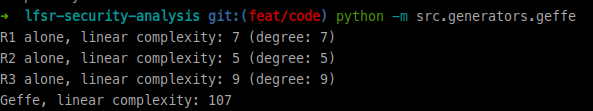
\includegraphics[width=0.9\textwidth]{images/execution_geffe.png}
\caption{Salida de \texttt{python -m src.generators.geffe}.}
\label{fig:exec-geffe}
\end{figure}

La complejidad lineal pasa de los grados originales (7, 5, 9) a 107. Hay una mejora clara, pero como veremos a continuación,
la complejidad lineal alta no salva al generador.

\subsection{La debilidad real, correlación}

El problema del generador de Geffe no es la complejidad lineal sino la correlación entre la salida y los LFSR internos.
Si miramos cuántas veces coincide la salida $s$ con $R_2$,

\[
  \Pr[s = b] = \Pr[s = b \mid a = 1]\Pr[a = 1] + \Pr[s = b \mid a = 0]\Pr[a = 0]
  = 1 \cdot \tfrac{1}{2} + \tfrac{1}{2} \cdot \tfrac{1}{2} = \tfrac{3}{4}
\]

La salida coincide con $R_2$ el 75\% de las veces. Lo mismo pasa con $R_3$.
Un atacante con un fragmento de keystream puede probar todos los estados posibles de $R_2$
(solo $2^5 = 32$ para nuestro ejemplo) y quedarse con el que produce coincidencia $\sim 75\%$.
Repite con $R_3$ y deduce $R_1$ a partir de los dos.

El coste total pasa de $2^{n_1 + n_2 + n_3}$ (fuerza bruta completa) a $2^{n_1} + 2^{n_2} + 2^{n_3}$, mucho menor.
Para nuestros tamaños son $2^7 + 2^5 + 2^9 = 672$ operaciones frente a $2^{21} \approx 2$ millones.
Y la correlación de $0{,}75$ no depende del tamaño de los registros, así que da igual usar LFSR de grado 100,
la vulnerabilidad sigue ahí.

Por esta razón el generador de Geffe se rompió conceptualmente con los ataques de correlación
de Siegenthaler~\cite{siegenthaler1985} y hoy no se usaría en producción.
En este trabajo sirve como caso base, ya que es el ejemplo perfecto de
que una complejidad lineal alta no basta si la función de combinación tiene correlación con sus entradas.

\section{Generador Shrinking}
\label{sec:shrinking}

El generador Shrinking, propuesto por Coppersmith, Krawczyk y Mansour~\cite{coppersmith1993}, funciona de forma completamente distinta a Geffe.
En vez de combinar las salidas con una función booleana, usa un registro para decidir qué bits del otro se incluyen en la salida y cuáles se tiran.

Los dos LFSR avanzan a la vez en cada ciclo,

\[
  s_i = \begin{cases} b_i & \text{si } a_i = 1 \\ \text{se descarta} & \text{si } a_i = 0 \end{cases}
\]

La consecuencia importante es que la secuencia de salida pierde la relación temporal con el reloj interno.
Un atacante que observe la secuencia no sabe cuántos ciclos han pasado entre dos bits consecutivos,
ya que no sabe cuántos se descartaron por el camino. Esto es lo que hace tan difícil aplicar Berlekamp-Massey directamente,
la secuencia que ve el atacante no es la salida directa de ningún LFSR, sino un muestreo irregular de uno.

\subsection{Ejemplo}

\begin{itemize}
  \item $R_1$ (selector), grado 3, polinomio $x^3 + x + 1$, estado $(1, 0, 1)$.
  \item $R_2$ (datos), grado 4, polinomio $x^4 + x + 1$, estado $(1, 1, 0, 0)$.
\end{itemize}

\begin{center}
\begin{tabular}{c|cc|c|l}
\hline
$t$ & $a$ ($R_1$) & $b$ ($R_2$) & Salida & Acción \\
\hline
1 & 1 & 0 & 0 & $a=1$, incluir $b$ \\
2 & 0 & 0 & --- & $a=0$, descartar \\
3 & 1 & 1 & 1 & $a=1$, incluir $b$ \\
4 & 1 & 1 & 1 & $a=1$, incluir $b$ \\
5 & 0 & 0 & --- & $a=0$, descartar \\
6 & 1 & 1 & 1 & $a=1$, incluir $b$ \\
7 & 0 & 0 & --- & $a=0$, descartar \\
8 & 1 & 0 & 0 & $a=1$, incluir $b$ \\
\hline
\end{tabular}
\end{center}

De 8 ciclos salen 5 bits, $\{0, 1, 1, 1, 0\}$.
Como $R_1$ produce aproximadamente la mitad de unos, de media se necesitan 2 ciclos por bit de salida.

\subsection{Implementación}

\begin{lstlisting}[style=Python,caption={Generador Shrinking (\texttt{src/generators/shrinking.py}).}]
def shrinking_generator(r1: LFSR, r2: LFSR, n: int) -> list[int]:
    """Generates n bits. r1 filters the output of r2."""
    output = []
    max_clocks = n * 10
    clocked = 0

    while len(output) < n and clocked < max_clocks:
        a = r1.next_bit()
        b = r2.next_bit()
        clocked += 1
        if a == 1:
            output.append(b)

    if len(output) < n:
        raise RuntimeError(
            f"could not generate {n} bits after {max_clocks} clocks"
        )

    return output
\end{lstlisting}

El parámetro \texttt{max\_clocks} es una protección, si por algún motivo $R_1$ produjera demasiados ceros consecutivos,
el bucle terminaría con un error en vez de quedarse colgado.

\subsection{Complejidad lineal}

Ejecutamos el generador con los mismos parámetros que antes,
$R_1$ grado 7 y $R_2$ grado 5, generando 1000 bits.

\begin{figure}[H]
\centering
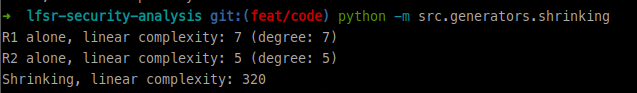
\includegraphics[width=0.9\textwidth]{images/execution_shrinking.png}
\caption{Salida de \texttt{python -m src.generators.shrinking}.}
\label{fig:exec-shrinking}
\end{figure}

El salto es espectacular. De LFSR de grados 7 y 5 (que individualmente tendrían complejidad lineal 7 y 5),
salimos con una complejidad lineal de 320. El factor de mejora frente al LFSR más grande es de unos 45x.
Y a diferencia de Geffe, no hay correlación directa explotable, ya que un atacante no sabe en qué posición del ciclo de $R_2$ está cada bit de la salida.

\subsection{Consideraciones prácticas}

La debilidad principal del Shrinking es que la seguridad depende de que $R_1$ sea desconocido.
Si alguien adivinara la secuencia de selección, sabría qué bits de $R_2$ forman la salida y aplicaría Berlekamp-Massey directamente.
El coste de esa fuerza bruta es $2^{n_1}$, así que se recomienda usar $n_1$ de al menos 64 bits en aplicaciones reales.

La otra consideración es la tasa de generación, no es constante, ya que cada bit de salida cuesta de media 2 ciclos de reloj.
En software esto no importa, basta llamar al generador en un bucle hasta tener los bits necesarios.
En hardware sí complica el diseño, hay que añadir un buffer entre el generador y el dispositivo que consume los bits para mantener una tasa de salida fija.

\section{Generador Self-Shrinking}
\label{sec:self-shrinking}

El Self-Shrinking, propuesto por Meier y Staffelbach~\cite{meier1994}, es una variante del Shrinking que usa un solo LFSR.
La idea es la misma (selección irregular) pero aplicada sobre la propia secuencia del registro.

Se toman los bits del LFSR de dos en dos. En cada par $(a, b)$, si $a = 1$ el bit $b$ pasa a la salida,
y si $a = 0$ se descartan los dos. La ventaja es que solo hace falta un registro.
La desventaja es que la tasa baja a un bit cada 4 ciclos (cada par consume 2 ciclos y solo la mitad de los pares producen salida).

\subsection{Ejemplo}

Un LFSR de grado 4 con polinomio $x^4 + x + 1$ y estado $(1, 1, 0, 0)$.

\begin{center}
\begin{tabular}{c|cc|c|l}
\hline
Par & $a$ & $b$ & Salida & Acción \\
\hline
1 & 0 & 0 & --- & $a=0$, descartar \\
2 & 1 & 1 & 1 & $a=1$, incluir $b$ \\
3 & 0 & 0 & --- & $a=0$, descartar \\
4 & 1 & 1 & 1 & $a=1$, incluir $b$ \\
5 & 0 & 1 & --- & $a=0$, descartar \\
6 & 0 & 0 & --- & $a=0$, descartar \\
7 & 1 & 0 & 0 & $a=1$, incluir $b$ \\
8 & 1 & 0 & 0 & $a=1$, incluir $b$ \\
\hline
\end{tabular}
\end{center}

16 bits del LFSR (8 pares) dan 4 bits de salida, $\{1, 1, 0, 0\}$.

\subsection{Implementación}

\begin{lstlisting}[style=Python,caption={Generador Self-Shrinking (\texttt{src/generators/self\_shrinking.py}).}]
def self_shrinking_generator(r: LFSR, n: int) -> list[int]:
    """Generates n bits from a single LFSR using self-shrinking."""
    output = []
    max_clocks = n * 10
    clocked = 0

    while len(output) < n and clocked < max_clocks:
        a = r.next_bit()
        b = r.next_bit()
        clocked += 2
        if a == 1:
            output.append(b)

    if len(output) < n:
        raise RuntimeError(
            f"could not generate {n} bits after {max_clocks} clocks"
        )

    return output
\end{lstlisting}

\subsection{Complejidad lineal}

Ejecutamos sobre un LFSR de grado 11 con polinomio $x^{11} + x^2 + 1$, generando 1000 bits.

\begin{figure}[H]
\centering
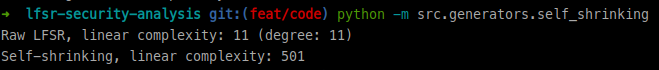
\includegraphics[width=0.9\textwidth]{images/execution_self_shrinking.png}
\caption{Salida de \texttt{python -m src.generators.self\_shrinking}.}
\label{fig:exec-self-shrinking}
\end{figure}

De nuevo el salto es enorme, de 11 a 501, factor 45x. La complejidad lineal queda en valores similares al Shrinking con menos hardware.

\subsection{Diferencias con el Shrinking}

Aunque el mecanismo de fondo es el mismo, hay una diferencia importante.
En Shrinking, el selector ($R_1$) y los datos ($R_2$) son LFSR completamente independientes, con polinomios y estados distintos.
En Self-Shrinking los bits de selección y los bits de datos son bits consecutivos del mismo LFSR,
así que están relacionados por la recurrencia del registro.
Es una debilidad teórica, difícil de explotar en la práctica pero que existe.
Por eso para el mismo nivel de seguridad se recomienda usar un LFSR de mayor grado que en Shrinking.

\section{Alternating Step Generator (ASG)}
\label{sec:asg}

El ASG fue propuesto por Günther~\cite{gunther1987} y es el más elaborado de los cuatro generadores.
Usa tres LFSR como Geffe, pero la forma de combinarlos es muy distinta.

En cada ciclo se avanza el registro de control $R_1$ y se lee su bit de salida.
Si es 1 se avanza $R_2$ (y $R_3$ se queda quieto), y si es 0 se avanza $R_3$ (y $R_2$ se queda quieto).
La salida del generador es el XOR de los bits actuales de $R_2$ y $R_3$, independientemente de cuál haya avanzado en ese ciclo.

\[
  s_i = b_2 \oplus b_3
\]

donde $b_2$ y $b_3$ son los bits más recientes de $R_2$ y $R_3$.

Es interesante comparar esto con Geffe, ya que ambos usan tres LFSR pero con resultados muy distintos.
En Geffe los tres registros avanzan siempre, y la salida depende directamente de cada uno en cada instante.
Eso es lo que permite la correlación. En ASG, $R_2$ y $R_3$ no avanzan a la vez, sino que uno se queda parado mientras el otro avanza,
y la decisión la toma $R_1$. Esto rompe la sincronización temporal entre la salida y cada registro individual.
Además la salida es el XOR de ambos (no una selección), lo que mezcla las dos secuencias de forma más profunda.

\subsection{Ejemplo}

\begin{itemize}
  \item $R_1$ (control), grado 3, polinomio $x^3 + x + 1$, estado $(1, 0, 1)$.
  \item $R_2$, grado 4, polinomio $x^4 + x + 1$, estado $(1, 1, 0, 0)$.
  \item $R_3$, grado 5, polinomio $x^5 + x^2 + 1$, estado $(1, 0, 1, 1, 0)$.
\end{itemize}

Al inicio se extraen los primeros bits de $R_2$ y $R_3$, $b_2 = 0$ y $b_3 = 0$.

\begin{center}
\begin{tabular}{c|c|cc|c|l}
\hline
$t$ & $a$ ($R_1$) & $b_2$ & $b_3$ & $s = b_2 \oplus b_3$ & Acción \\
\hline
1 & 1 & 0 & 0 & 0 & Avanza $R_2$, $b_2 \leftarrow 0$ \\
2 & 0 & 0 & 0 & 1 & Avanza $R_3$, $b_3 \leftarrow 1$ \\
3 & 1 & 0 & 1 & 0 & Avanza $R_2$, $b_2 \leftarrow 1$ \\
4 & 1 & 1 & 1 & 0 & Avanza $R_2$, $b_2 \leftarrow 1$ \\
5 & 0 & 1 & 1 & 1 & Avanza $R_3$, $b_3 \leftarrow 0$ \\
6 & 1 & 1 & 0 & 0 & Avanza $R_2$, $b_2 \leftarrow 0$ \\
7 & 0 & 0 & 0 & 1 & Avanza $R_3$, $b_3 \leftarrow 1$ \\
8 & 1 & 0 & 1 & 1 & Avanza $R_2$, $b_2 \leftarrow 0$ \\
\hline
\end{tabular}
\end{center}

La salida es $\{0, 1, 0, 0, 1, 0, 1, 1, \ldots\}$.

\subsection{Implementación}

\begin{lstlisting}[style=Python,caption={Generador ASG (\texttt{src/generators/alternating\_step.py}).}]
def alternating_step_generator(r1: LFSR, r2: LFSR, r3: LFSR, n: int) -> list[int]:
    """Generates n bits. r1 decides which of r2/r3 advances."""
    output = []

    b2 = r2.next_bit()
    b3 = r3.next_bit()

    for _ in range(n):
        a = r1.next_bit()
        if a == 1:
            b2 = r2.next_bit()
        else:
            b3 = r3.next_bit()
        output.append(b2 ^ b3)

    return output
\end{lstlisting}

Una sutileza, los bits $b_2$ y $b_3$ se inicializan fuera del bucle. Esto es necesario porque en cada iteración solo se avanza uno de los dos,
así que el otro tiene que tener un valor previo válido para entrar en el XOR.

\subsection{Complejidad lineal}

Ejecutamos el generador con los mismos LFSR que usamos en Geffe,
grados 7, 5 y 9 con 1000 bits de salida.

\begin{figure}[H]
\centering
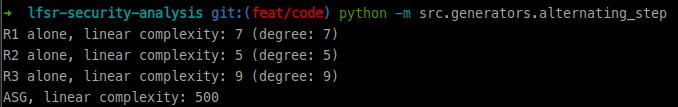
\includegraphics[width=0.9\textwidth]{images/execution_alternating_step.png}
\caption{Salida de \texttt{python -m src.generators.alternating\_step}.}
\label{fig:exec-asg}
\end{figure}

Esto es lo más interesante de todo el capítulo. Con los mismos LFSR que dieron 107 de complejidad lineal en Geffe,
el ASG llega a 500. La diferencia no está en los registros ni en sus tamaños sino exclusivamente
en cómo se combinan sus salidas. Reloj alterno y XOR de fuentes independientes amplifica mucho más la complejidad lineal que un multiplexor.

\subsection{Seguridad}

El ASG combina dos defensas a la vez, reloj irregular (un atacante no sabe cuántas veces avanzó cada registro)
y XOR de dos fuentes (aunque supiera el control $R_1$, todavía tendría que romper $R_2$ y $R_3$ a la vez).
No se conocen ataques de correlación prácticos cuando los registros son lo bastante grandes.

El mejor ataque conocido tiene coste del orden de $2^{n_2 + n_3}$,
fuerza bruta sobre los dos registros de datos en paralelo.
Con $n_2$ y $n_3$ de 64 bits cada uno, el ataque tiene coste $2^{128}$, que se considera fuera del alcance computacional actual.

\section{Resumen comparativo}

La tabla siguiente compara los cuatro generadores con los parámetros que vamos a usar en el análisis experimental del capítulo siguiente.

\begin{center}
\begin{tabular}{l|cccc}
\hline
& Geffe & Shrinking & Self-Shrinking & ASG \\
\hline
LFSR usados & 3 & 2 & 1 & 3 \\
Mecanismo & Multiplexor & Selección & Auto-selección & Reloj alterno \\
Ciclos por bit & 1 & $\sim 2$ & $\sim 4$ & 1 \\
LC sobre 1000 bits & 107 & 320 & 501 & 500 \\
Correlación con LFSR & 0,75 & No directa & No directa & No directa \\
\hline
\end{tabular}
\end{center}

Tres observaciones rápidas.

Primero, Geffe es el caso débil. Su complejidad lineal es menor que la de los otros tres (un orden de magnitud por debajo) y además tiene correlación 0,75,
lo que permite ataques mucho más eficientes que Berlekamp-Massey.

Segundo, Shrinking, Self-Shrinking y ASG quedan en complejidades lineales parecidas (320, 501, 500) con secuencias de 1000 bits.
En el capítulo siguiente, con secuencias más largas, se sigue manteniendo esta proximidad y los tres se acercan a $N/2$.

Tercero, comparando Geffe y ASG (que usan los mismos tres LFSR), la diferencia entre 107 y 500 sale solo del mecanismo de combinación.
Mismo hardware, conexión distinta, resultado completamente distinto. Esto es probablemente la lección más importante del trabajo,
en generadores basados en LFSR la clave no es el tamaño de los registros sino cómo se combinan.

El capítulo siguiente lleva todo esto un paso más allá, ejecuta los cuatro generadores con secuencias más largas, mide su complejidad lineal exacta
y los pasa por ocho tests estadísticos del estándar NIST para ver qué generador tiene la mejor calidad de salida en la práctica.


\chapter{Análisis experimental}
\label{cap:analisis}

Este capítulo presenta los resultados de pasar los cuatro generadores por una batería de tests estadísticos del estándar NIST SP 800-22~\cite{nist2010}
y de medir la complejidad lineal de las secuencias que producen. La idea no es solo ver qué generadores ``pasan'' y cuáles ``fallan'',
sino entender el porqué y conectarlo con la teoría de los capítulos anteriores.

Para cada test se describe brevemente qué evalúa, se incluye el código real que lo implementa, y se aplica sobre las secuencias generadas.
Al final del capítulo se presenta la tabla consolidada de resultados, las gráficas de comparación y un análisis por generador.

\section{Configuración experimental}

Cada generador se ejecuta con LFSR de polinomios primitivos sobre $\{0, 1\}$ y estados iniciales fijos (distintos de cero) para asegurar reproducibilidad.
Los LFSR usados son los siguientes, todos con polinomios primitivos.

\begin{itemize}
  \item LFSR puro de grado 19, polinomio $x^{19} + x^{5} + x^2 + x + 1$.
  \item LFSR auxiliar de grado 17, polinomio $x^{17} + x^3 + 1$.
  \item LFSR auxiliar de grado 15, polinomio $x^{15} + x + 1$.
\end{itemize}

Cada generador se construye con combinaciones de estos registros. Shrinking usa el de grado 19 como selector y el de 17 como datos.
Self-Shrinking usa solo el de grado 19. Geffe y ASG usan los tres.

Se generan secuencias de \textbf{500.000 bits} para los tests NIST
(la mayoría de tests necesitan secuencias largas para tener potencia estadística suficiente, en particular Maurer y el de complejidad lineal por bloques).
Sobre esas secuencias, la complejidad lineal global se calcula con Berlekamp-Massey sobre los primeros 5.000 bits, ya que el algoritmo es $O(N^2)$
y procesar medio millón de bits tardaría horas.

El nivel de significación para todos los tests es $\alpha = 0{,}01$. Un p-valor mayor o igual a $0{,}01$ se considera que pasa el test,
y un p-valor menor que el generador tiene una debilidad estadística detectable en esa propiedad.

\section{Tests aplicados}

De los quince tests del estándar NIST SP 800-22 se implementan ocho.
Los siete restantes (cumulative sums, random excursions y variantes, approximate entropy,
overlapping template matching y longest run of ones) requieren secuencias considerablemente más largas
o evalúan propiedades que en el contexto de LFSR son redundantes con las que ya cubrimos.

\subsection{Test de frecuencia (Monobit)}

Comprueba si la proporción de unos y ceros en la secuencia se acerca al 50\%.
El estadístico convierte los bits a $\pm 1$, los suma y mira si el resultado está cerca de cero.

\begin{lstlisting}[style=Python,caption={Test Monobit (\texttt{src/tests\_nist/monobit.py}).}]
def monobit_test(sequence: list[int]) -> tuple[float, bool]:
    n = len(sequence)
    if n < 100:
        raise ValueError("sequence too short, need at least 100 bits")

    S_n = sum(1 if b == 1 else -1 for b in sequence)
    s_obs = abs(S_n) / math.sqrt(n)
    p_value = math.erfc(s_obs / math.sqrt(2))

    return p_value, p_value >= 0.01
\end{lstlisting}

Es el test más básico, si una secuencia tiene un sesgo claro hacia uno de los dos valores,
este test lo detecta. Pasarlo es condición necesaria pero está lejos de ser suficiente.

\subsection{Test de frecuencia en bloques}

Versión más detallada del monobit. Divide la secuencia en bloques de longitud $M$ y comprueba si la proporción de unos dentro de cada bloque se acerca a $1/2$.
Detecta desequilibrios locales que el monobit global no vería.

\begin{lstlisting}[style=Python,caption={Test Block Frequency (\texttt{src/tests\_nist/block\_frequency.py}).}]
def block_frequency_test(sequence: list[int], block_size: int = 128) -> tuple[float, bool]:
    n = len(sequence)
    num_blocks = n // block_size

    proportions = []
    for i in range(num_blocks):
        block = sequence[i * block_size : (i + 1) * block_size]
        pi_i = sum(block) / block_size
        proportions.append(pi_i)

    chi_sq = 4 * block_size * sum((pi - 0.5) ** 2 for pi in proportions)
    p_value = _igamc(num_blocks / 2, chi_sq / 2)

    return p_value, p_value >= 0.01
\end{lstlisting}

En los experimentos uso bloques de 128 bits, que es el valor recomendado por defecto del estándar.

\subsection{Test de rachas}

Una racha es una subsecuencia maximal de bits consecutivos iguales,
por ejemplo en $\{1, 1, 0, 0, 0, 1\}$ hay tres rachas.
El test comprueba si el número total de rachas es coherente con una secuencia aleatoria.
Demasiadas rachas indican oscilación excesiva, pocas indican bloques largos de bits iguales.

\begin{lstlisting}[style=Python,caption={Test de rachas (\texttt{src/tests\_nist/runs.py}).}]
def runs_test(sequence: list[int]) -> tuple[float, bool]:
    n = len(sequence)
    pi = sum(sequence) / n

    tau = 2 / math.sqrt(n)
    if abs(pi - 0.5) >= tau:
        return 0.0, False

    V_n = 1 + sum(
        1 for k in range(n - 1) if sequence[k] != sequence[k + 1]
    )

    numerator = abs(V_n - 2 * n * pi * (1 - pi))
    denominator = 2 * math.sqrt(2 * n) * pi * (1 - pi)
    p_value = math.erfc(numerator / denominator)

    return p_value, p_value >= 0.01
\end{lstlisting}

El test tiene un prerrequisito de balance, si la proporción de unos está muy lejos de $0{,}5$,
no tiene sentido calcular el estadístico y se devuelve p-valor 0 directamente.

\subsection{Test de rango de matriz binaria}

Toma chunks consecutivos de la secuencia, los reorganiza en matrices $32 \times 32$ y calcula su rango con XOR.
En una secuencia aleatoria, las matrices tienden a tener rango completo con una probabilidad conocida.
En secuencias con estructura lineal el rango es menor.

\begin{lstlisting}[style=Python,caption={Test Binary Matrix Rank (extracto de \texttt{src/tests\_nist/binary\_matrix.py}).}]
def binary_matrix_rank_test(sequence: list[int], rows: int = 32, cols: int = 32):
    n = len(sequence)
    block_size = rows * cols
    num_matrices = n // block_size

    F_M = 0; F_M1 = 0; F_rem = 0
    for i in range(num_matrices):
        block = sequence[i * block_size : (i + 1) * block_size]
        matrix = [block[r * cols : (r + 1) * cols] for r in range(rows)]
        rank = _gf2_rank(matrix)

        if rank == rows:
            F_M += 1
        elif rank == rows - 1:
            F_M1 += 1
        else:
            F_rem += 1

    chi_sq = (
        (F_M - num_matrices * 0.2888) ** 2 / (num_matrices * 0.2888) +
        (F_M1 - num_matrices * 0.5776) ** 2 / (num_matrices * 0.5776) +
        (F_rem - num_matrices * 0.1336) ** 2 / (num_matrices * 0.1336)
    )
    p_value = math.exp(-chi_sq / 2)
    return p_value, p_value >= 0.01
\end{lstlisting}

Este test es especialmente relevante para LFSR, ya que un LFSR de grado $n$ con $n < 32$ tiende a producir matrices con dependencias lineales entre filas
(las filas viven en un subespacio de dimensión a lo sumo $n$), lo que reduce el rango y dispara el chi-cuadrado.

\subsection{Test universal de Maurer}

Mide la compresibilidad de la secuencia. La idea intuitiva es que una secuencia verdaderamente aleatoria no se puede comprimir significativamente porque no hay patrones que aprovechar.
Si la secuencia tiene regularidades (periodicidad, correlaciones a larga distancia), los patrones se repiten con más frecuencia de la esperada.

\begin{lstlisting}[style=Python,caption={Test universal de Maurer (extracto, \texttt{src/tests\_nist/maurer.py}).}]
def maurer_test(sequence: list[int], block_size: int = 7) -> tuple[float, bool]:
    L = block_size
    Q = 10 * (2 ** L)
    n = len(sequence)
    K = n // L - Q

    T = [0] * (2 ** L)
    for i in range(Q):
        block = sequence[i * L : (i + 1) * L]
        idx = int("".join(str(b) for b in block), 2)
        T[idx] = i + 1

    sum_log = 0.0
    for i in range(Q, Q + K):
        block = sequence[i * L : (i + 1) * L]
        idx = int("".join(str(b) for b in block), 2)
        distance = (i + 1) - T[idx]
        sum_log += math.log2(distance)
        T[idx] = i + 1

    f_n = sum_log / K
    expected, variance = _MAURER_TABLE[L]
    c = 0.7 - 0.8 / L + (4 + 32 / L) * (K ** (-3.0 / L)) / 15
    sigma = c * math.sqrt(variance / K)

    p_value = math.erfc(abs(f_n - expected) / (math.sqrt(2) * sigma))
    return p_value, p_value >= 0.01
\end{lstlisting}

En los experimentos uso $L = 6$ que es el valor mínimo recomendado para secuencias del orden de medio millón de bits.

\subsection{Test serial}

Comprueba que todos los patrones de $m$ bits aparezcan con frecuencia similar. Para $m = 3$, los ocho patrones posibles ($000$, $001$, $\ldots$, $111$) deberían aparecer
aproximadamente con la misma frecuencia $1/8$ cada uno.

\begin{lstlisting}[style=Python,caption={Test serial (\texttt{src/tests\_nist/serial.py}).}]
def serial_test(sequence: list[int], block_size: int = 3):
    n = len(sequence)
    m = block_size

    psi_sq_m  = _psi_sq(sequence, n, m)
    psi_sq_m1 = _psi_sq(sequence, n, m - 1)
    psi_sq_m2 = _psi_sq(sequence, n, m - 2) if m >= 2 else 0.0

    del1 = psi_sq_m - psi_sq_m1
    del2 = psi_sq_m - 2 * psi_sq_m1 + psi_sq_m2

    p1 = float(gammaincc(2 ** (m - 2), del1 / 2))
    p2 = float(gammaincc(2 ** (m - 3), del2 / 2)) if m >= 2 else 1.0

    passed = p1 >= 0.01 and p2 >= 0.01
    return (p1, p2), passed
\end{lstlisting}

El test devuelve dos p-valores y los dos tienen que pasar. Para reportar un único valor en las tablas uso el mínimo de los dos.

\subsection{Test espectral (DFT)}

Aplica la transformada discreta de Fourier a la secuencia (convirtiendo previamente los bits a $\pm 1$) y mira si hay picos
anormalmente altos en el espectro de frecuencias, lo que indicaría periodicidades ocultas.

\begin{lstlisting}[style=Python,caption={Test espectral (\texttt{src/tests\_nist/spectral.py}).}]
def spectral_test(sequence: list[int]) -> tuple[float, bool]:
    n = len(sequence)
    x = np.array([1 if b == 1 else -1 for b in sequence], dtype=float)

    X = np.fft.fft(x)
    magnitudes = np.abs(X[: n // 2])

    threshold = math.sqrt(math.log(1 / 0.05) * n)
    N_0 = 0.95 * n / 2
    N_1 = np.sum(magnitudes < threshold)

    d = (N_1 - N_0) / math.sqrt(n * 0.95 * 0.05 / 4)
    p_value = math.erfc(abs(d) / math.sqrt(2))

    return p_value, p_value >= 0.01
\end{lstlisting}

Este test es el que más nos interesa en el contexto de LFSR, ya que las m-sequences tienen periodicidad perfecta y los generadores que muestrean LFSR
pueden conservar componentes frecuenciales del registro original. Como se verá en los resultados, es el test que mejor discrimina entre generadores.

\subsection{Test de complejidad lineal}

Divide la secuencia en bloques de longitud $M$, calcula la complejidad lineal de cada bloque con Berlekamp-Massey y compara la distribución de complejidades observadas
con la teórica para bloques aleatorios.

\begin{lstlisting}[style=Python,caption={Test de complejidad lineal (extracto, \texttt{src/tests\_nist/linear\_complexity.py}).}]
def linear_complexity_test(sequence: list[int], block_size: int = 500):
    n = len(sequence)
    M = block_size
    N = n // M

    mu = M / 2 + (9 + (-1) ** (M + 1)) / 36 - (M / 3 + 2 / 9) / (2 ** M)

    T = []
    for i in range(N):
        block = sequence[i * M : (i + 1) * M]
        L = linear_complexity(block)
        T.append((-1) ** M * (L - mu) + 2 / 9)

    nu = [0] * 7
    for t in T:
        if t <= -2.5: nu[0] += 1
        elif t <= -1.5: nu[1] += 1
        elif t <= -0.5: nu[2] += 1
        elif t <= 0.5: nu[3] += 1
        elif t <= 1.5: nu[4] += 1
        elif t <= 2.5: nu[5] += 1
        else: nu[6] += 1

    pi = [0.010417, 0.03125, 0.125, 0.5, 0.25, 0.0625, 0.020833]
    chi_sq = sum((nu[i] - N * pi[i]) ** 2 / (N * pi[i]) for i in range(7))
    p_value = float(gammaincc(3, chi_sq / 2))
    return p_value, p_value >= 0.01
\end{lstlisting}

Uso bloques de 500 bits, valor estándar. Es el test que tira de Berlekamp-Massey de forma directa,
y por eso el que detecta más limpiamente las secuencias con estructura lineal.

\section{Resultados}

\subsection{Salida de la ejecución}

El módulo \texttt{src.analysis.run\_experiments} genera las cinco secuencias (LFSR puro, Shrinking, Self-Shrinking, Geffe y ASG),
pasa cada una por los ocho tests, calcula la complejidad lineal y guarda todo en \texttt{results/results.json}.
Esta es la salida real de una ejecución completa.

\begin{figure}[H]
\centering
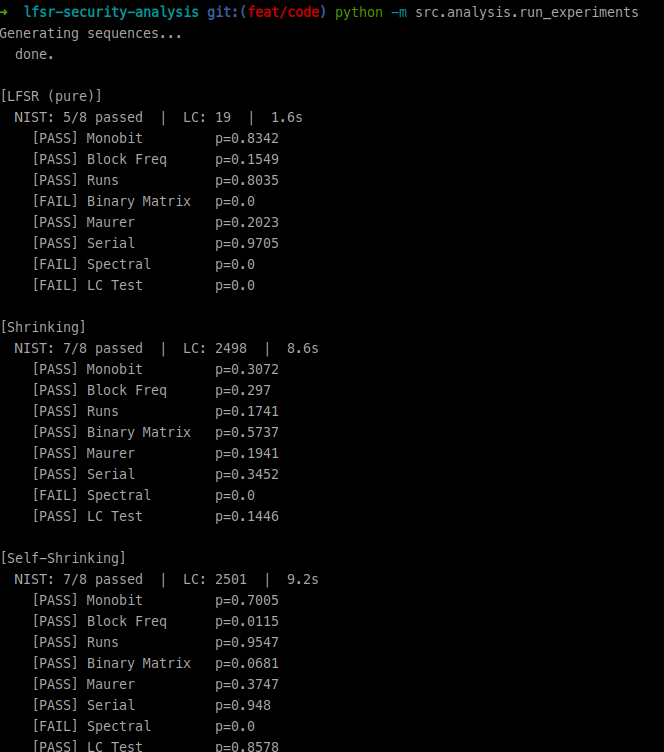
\includegraphics[width=0.9\textwidth]{images/execution_run_experiments_1.png}
\caption{Salida de \texttt{python -m src.analysis.run\_experiments} (parte 1).}
\label{fig:exec-run-experiments-1}
\end{figure}

\begin{figure}[H]
\centering
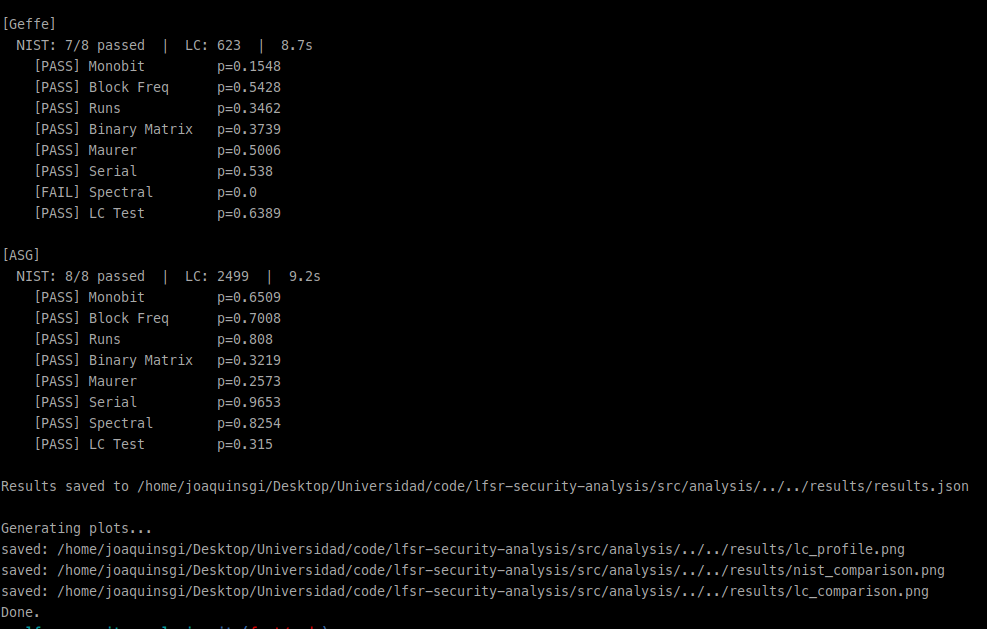
\includegraphics[width=0.9\textwidth]{images/execution_run_experiments_2.png}
\caption{Salida de \texttt{python -m src.analysis.run\_experiments} (parte 2).}
\label{fig:exec-run-experiments-2}
\end{figure}

Cada secuencia tarda unos 10-13 segundos en procesarse. El LFSR puro es el más rápido (1,8 s) porque cae directamente en tres tests sin necesidad de cálculos intensivos.

\subsection{Tabla consolidada}

La tabla~\ref{tab:nist} presenta los p-valores en formato compacto. Los valores en negrita son los que no pasan el umbral $\alpha = 0{,}01$.

\begin{table}[ht]
\centering
\begin{tabular}{l|ccccc}
\hline
\textbf{Test} & \textbf{LFSR} & \textbf{Shrinking} & \textbf{Self-Shr.} & \textbf{Geffe} & \textbf{ASG} \\
\hline
Monobit            & 0,834          & 0,307          & 0,701          & 0,155          & 0,651 \\
Block Freq.        & 0,155          & 0,297          & 0,012          & 0,543          & 0,701 \\
Runs               & 0,804          & 0,174          & 0,955          & 0,346          & 0,808 \\
Binary Matrix      & \textbf{0,000} & 0,574          & 0,068          & 0,374          & 0,322 \\
Maurer             & 0,202          & 0,194          & 0,375          & 0,501          & 0,257 \\
Serial             & 0,971          & 0,345          & 0,948          & 0,538          & 0,965 \\
Espectral          & \textbf{0,000} & \textbf{0,000} & \textbf{0,000} & \textbf{0,000} & 0,825 \\
Complejidad lineal & \textbf{0,000} & 0,145          & 0,858          & 0,639          & 0,315 \\
\hline
\textbf{Pasados}   & 5/8            & 7/8            & 7/8            & 7/8            & 8/8 \\
\textbf{LC medida} & 19             & 2498           & 2501           & 623            & 2499 \\
\hline
\end{tabular}
\caption{P-valores de los ocho tests NIST y complejidad lineal sobre 5.000 bits. Los valores en negrita ($< 0{,}01$) indican tests fallidos.}
\label{tab:nist}
\end{table}

\subsection{Gráficas}

La figura~\ref{fig:lc-bar} compara la complejidad lineal alcanzada por cada generador.
El LFSR puro y el generador de Geffe quedan claramente por debajo de los otros tres,
que se acercan al valor ideal de $N/2 = 2500$ para una secuencia aleatoria de 5.000 bits.

\begin{figure}[H]
\centering
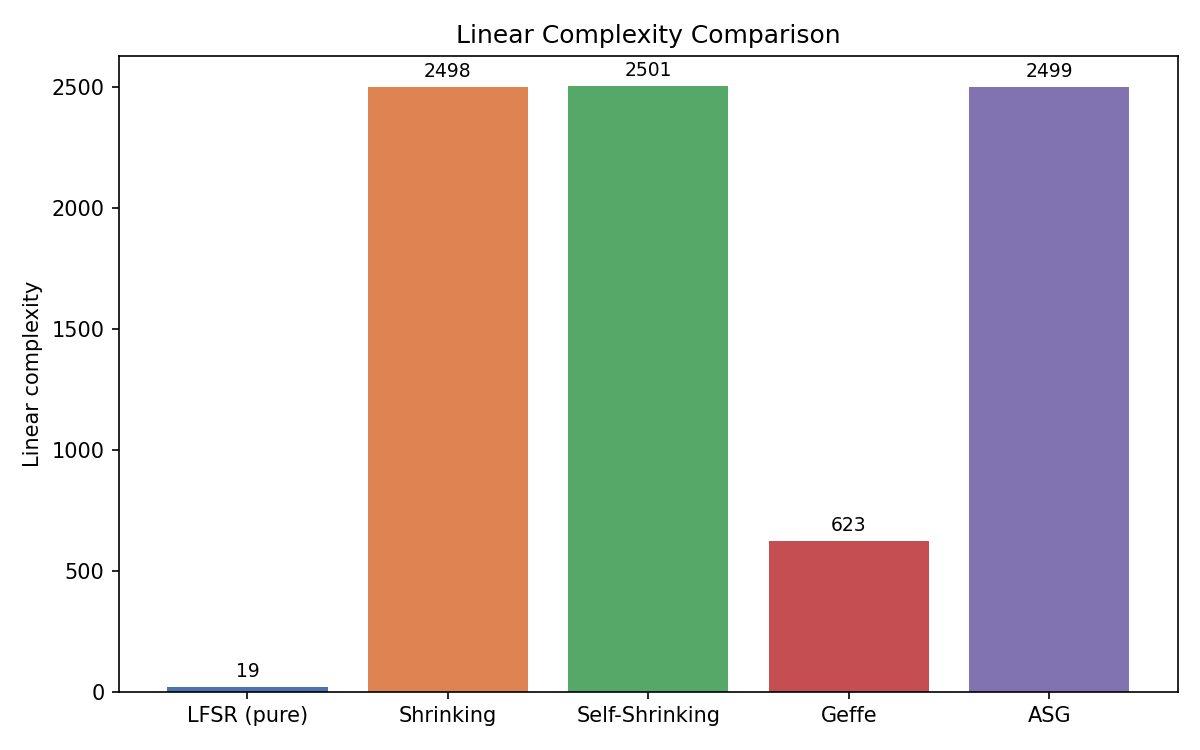
\includegraphics[width=0.8\textwidth]{images/lc_comparison.png}
\caption{Complejidad lineal de cada generador sobre secuencias de 5.000 bits.}
\label{fig:lc-bar}
\end{figure}

El perfil de complejidad lineal (figura~\ref{fig:lc-profile}) muestra cómo evoluciona la complejidad a medida que se procesan más bits.
El LFSR puro se estanca muy pronto en su grado (19), el generador de Geffe crece más despacio que el resto,
y Shrinking, Self-Shrinking y ASG siguen prácticamente la recta $N/2$ esperada de una secuencia aleatoria.

\begin{figure}[H]
\centering
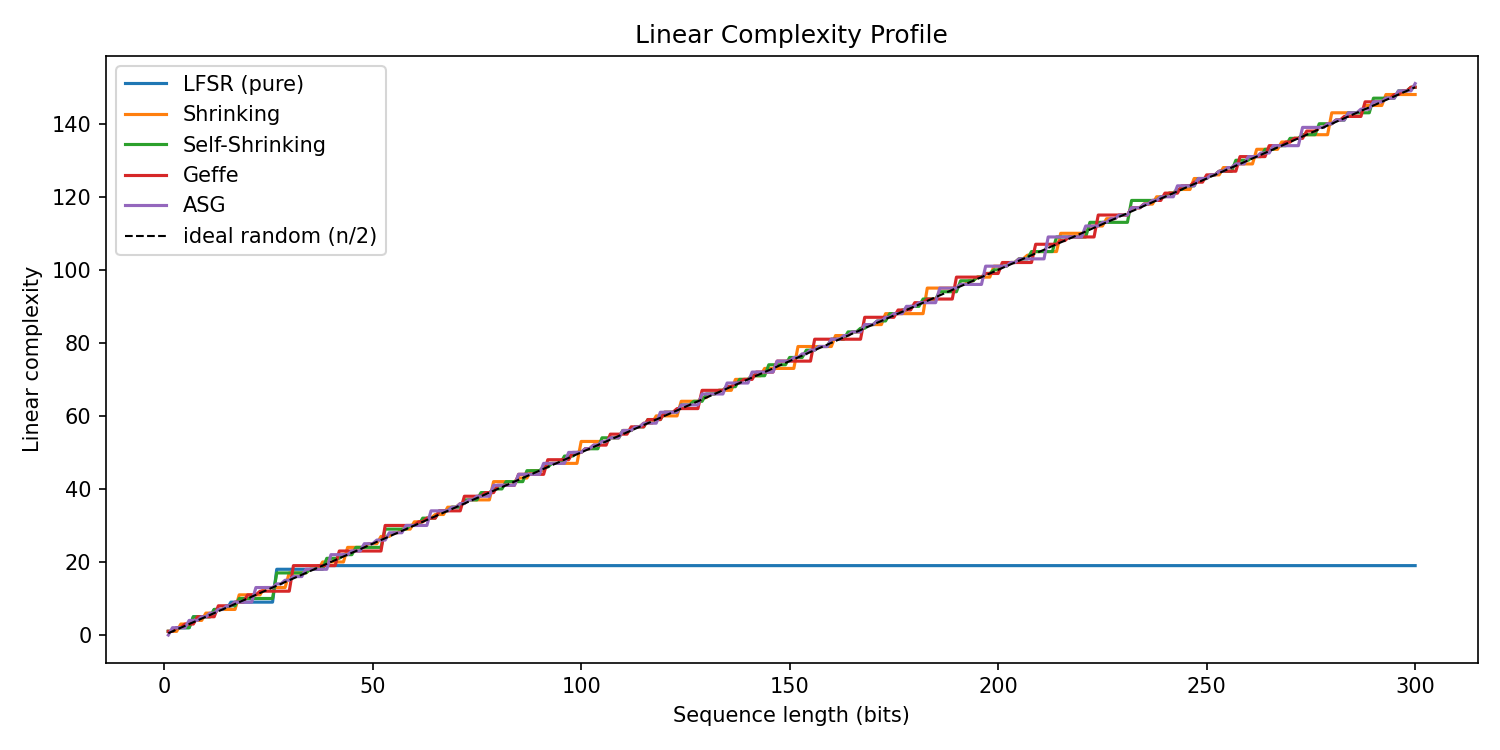
\includegraphics[width=0.85\textwidth]{images/lc_profile.png}
\caption{Perfil de complejidad lineal para los primeros 300 bits de cada generador.
La recta $N/2$ marca el comportamiento esperado de una secuencia aleatoria.}
\label{fig:lc-profile}
\end{figure}

La figura~\ref{fig:nist-comparison} muestra los p-valores de los ocho tests en formato visual.
El generador de ASG (verde) es el único cuyos p-valores se mantienen por encima del umbral en todos los tests. El resto cae en al menos uno.

\begin{figure}[H]
\centering
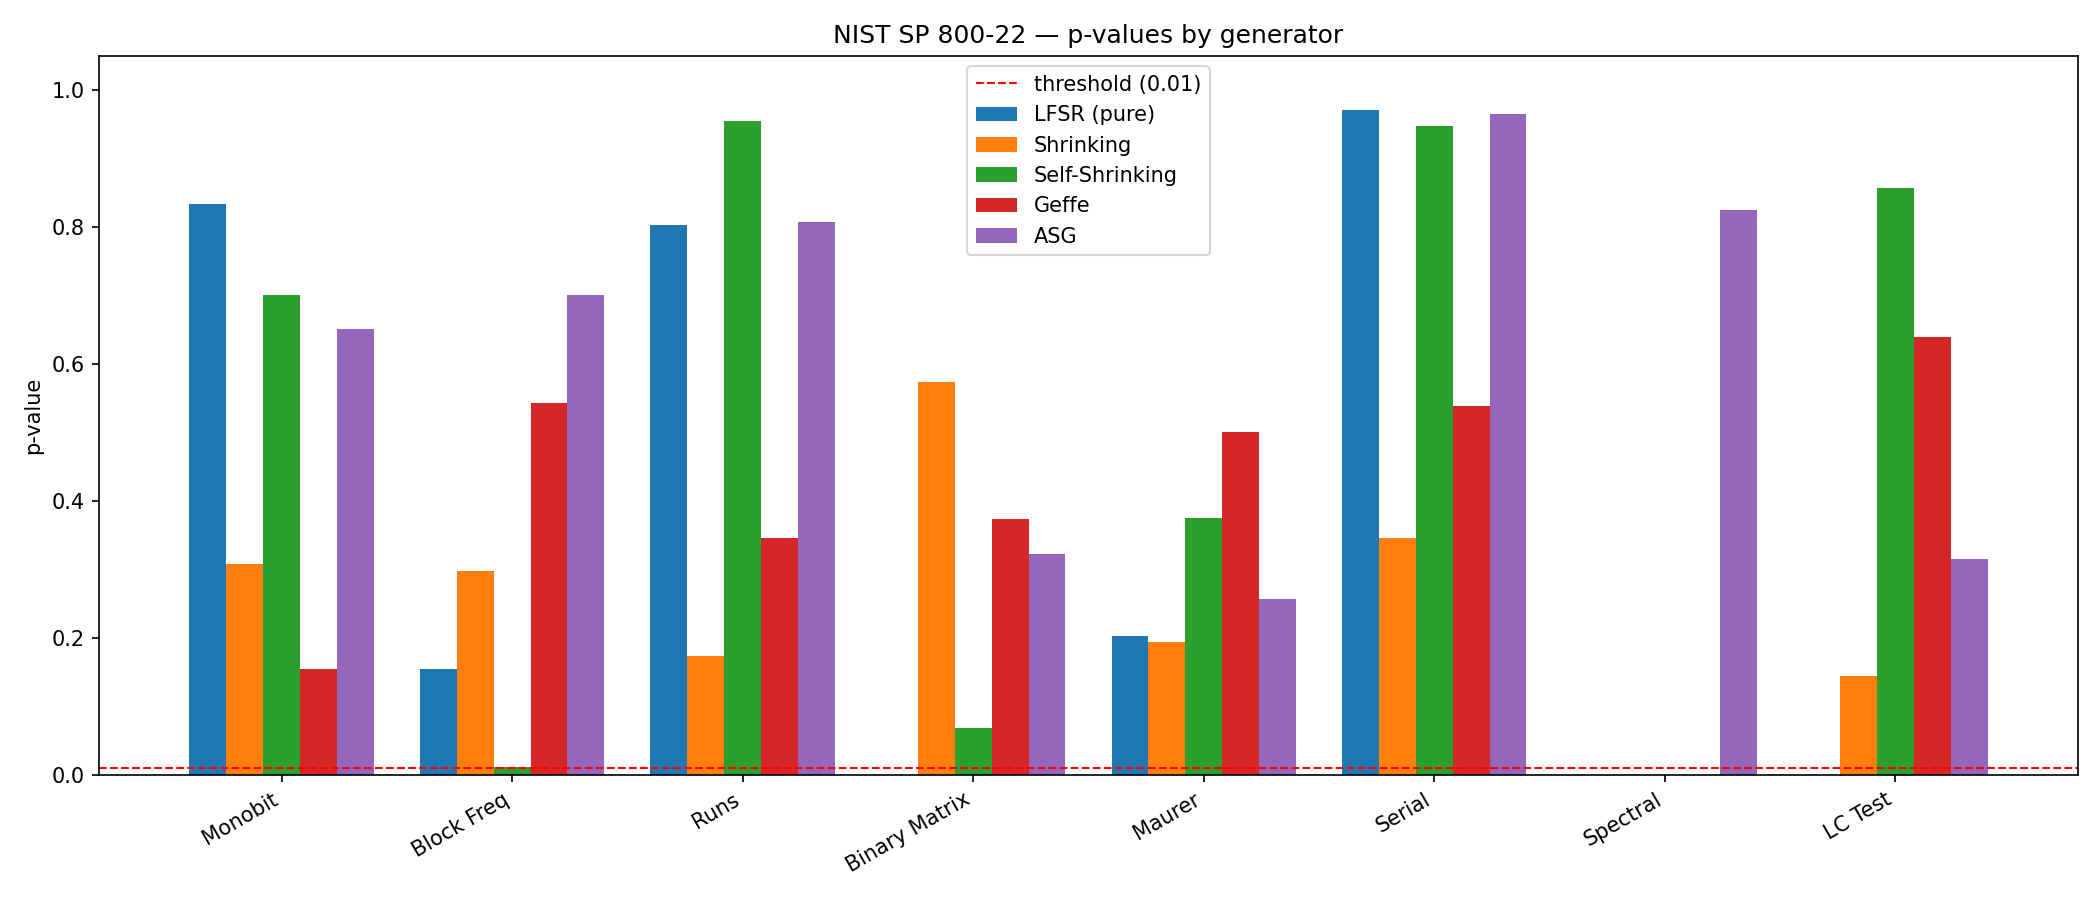
\includegraphics[width=0.95\textwidth]{images/nist_comparison.png}
\caption{P-valores por test y por generador. La línea punteada marca el umbral $\alpha = 0{,}01$.}
\label{fig:nist-comparison}
\end{figure}

\section{Comportamiento con distintos tamaños de secuencia}
\label{sec:multi-size}

Los resultados anteriores corresponden a una longitud de secuencia concreta.
Para ver cómo dependen del tamaño, repito los experimentos con $n \in \{1000, 5000, 10000, 50000\}$
midiendo la complejidad lineal y los p-valores de tres tests representativos,
Monobit (balance global), Runs (estructura local) y Espectral (periodicidad).

El script \texttt{multi\_size.py} hace exactamente eso, genera las cinco secuencias para cada $n$ y va imprimiendo los resultados en formato tabla.

\begin{figure}[H]
\centering
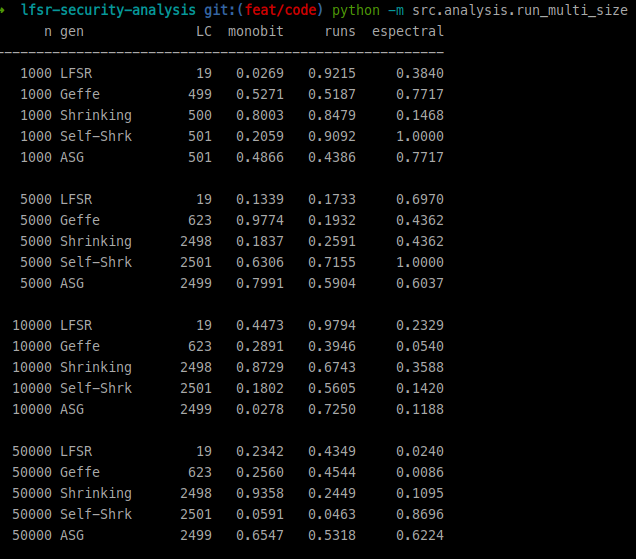
\includegraphics[width=0.9\textwidth]{images/execution_multi_size.png}
\caption{Salida de \texttt{python -m src.analysis.run\_multi\_size}.}
\label{fig:exec-multi-size}
\end{figure}

Hay tres patrones interesantes que se ven de un vistazo en estos datos.

Primero, la \textbf{complejidad lineal del LFSR puro se queda anclada en 19} por mucho que se alargue la secuencia.
Es exactamente lo que predice la teoría, da igual ver 1000 o 50000 bits, Berlekamp-Massey siempre devuelve el grado del registro.
Esa estabilidad es la firma de una secuencia lineal.

Segundo, los generadores no triviales saturan la complejidad lineal en valores cercanos a $N/2$.
Con $n = 1000$ todos rondan 500, con $n = 5000$ rondan 2500 (excepto Geffe, que se queda en 623).
La cota $\Lambda \leq \lfloor N/2 \rfloor$ se cumple siempre y se saturan a partir de cierta longitud porque la complejidad lineal se calcula sobre los primeros 5000 bits.

Tercero, el \textbf{test espectral se vuelve más estricto cuando la secuencia crece}.
Con $n = 1000$ casi cualquier generador lo pasa cómodamente. Con $n = 50000$, el LFSR puro y Geffe
empiezan a quedar peligrosamente cerca del umbral (0,024 y 0,0086 respectivamente),
y a partir de aquí esperaríamos que cayeran por debajo. Esto es coherente con lo que vimos antes en la tabla principal,
con secuencias de 500.000 bits los cuatro generadores excepto el ASG fallan el espectral con p-valor 0.

\section{Validación del software}
\label{sec:validacion}

Antes de fiarse de los p-valores reportados conviene verificar que el código no contiene errores.
Cada componente del repositorio tiene su batería de tests unitarios con \texttt{pytest},
que comprueba contra valores conocidos. Los tests cubren tres áreas.

\begin{itemize}
  \item \textbf{LFSR} (7 tests). Periodo máximo con polinomios primitivos de grado 5 y 7,
        salida binaria, reset del estado, validación de errores en el constructor
        (estado todo-ceros, longitud incorrecta, bits inválidos).
  \item \textbf{Berlekamp-Massey} (6 tests). Complejidad lineal de una m-sequence igual al grado del LFSR original,
        reconstrucción del LFSR a partir de $2n$ bits, secuencia constante con $\Lambda = 1$,
        secuencia alternante con $\Lambda = 2$, perfil de complejidad no decreciente,
        polinomio recuperado con $c_0 = 1$.
  \item \textbf{Generadores} (14 tests). Longitud de salida correcta, salida binaria,
        complejidad lineal mayor que la de los componentes y determinismo
        (la misma semilla produce la misma secuencia) para cada uno de los cuatro generadores.
\end{itemize}

Al ejecutar \texttt{pytest} sobre el árbol completo, los 27 tests pasan en menos de un segundo.

\begin{figure}[H]
\centering
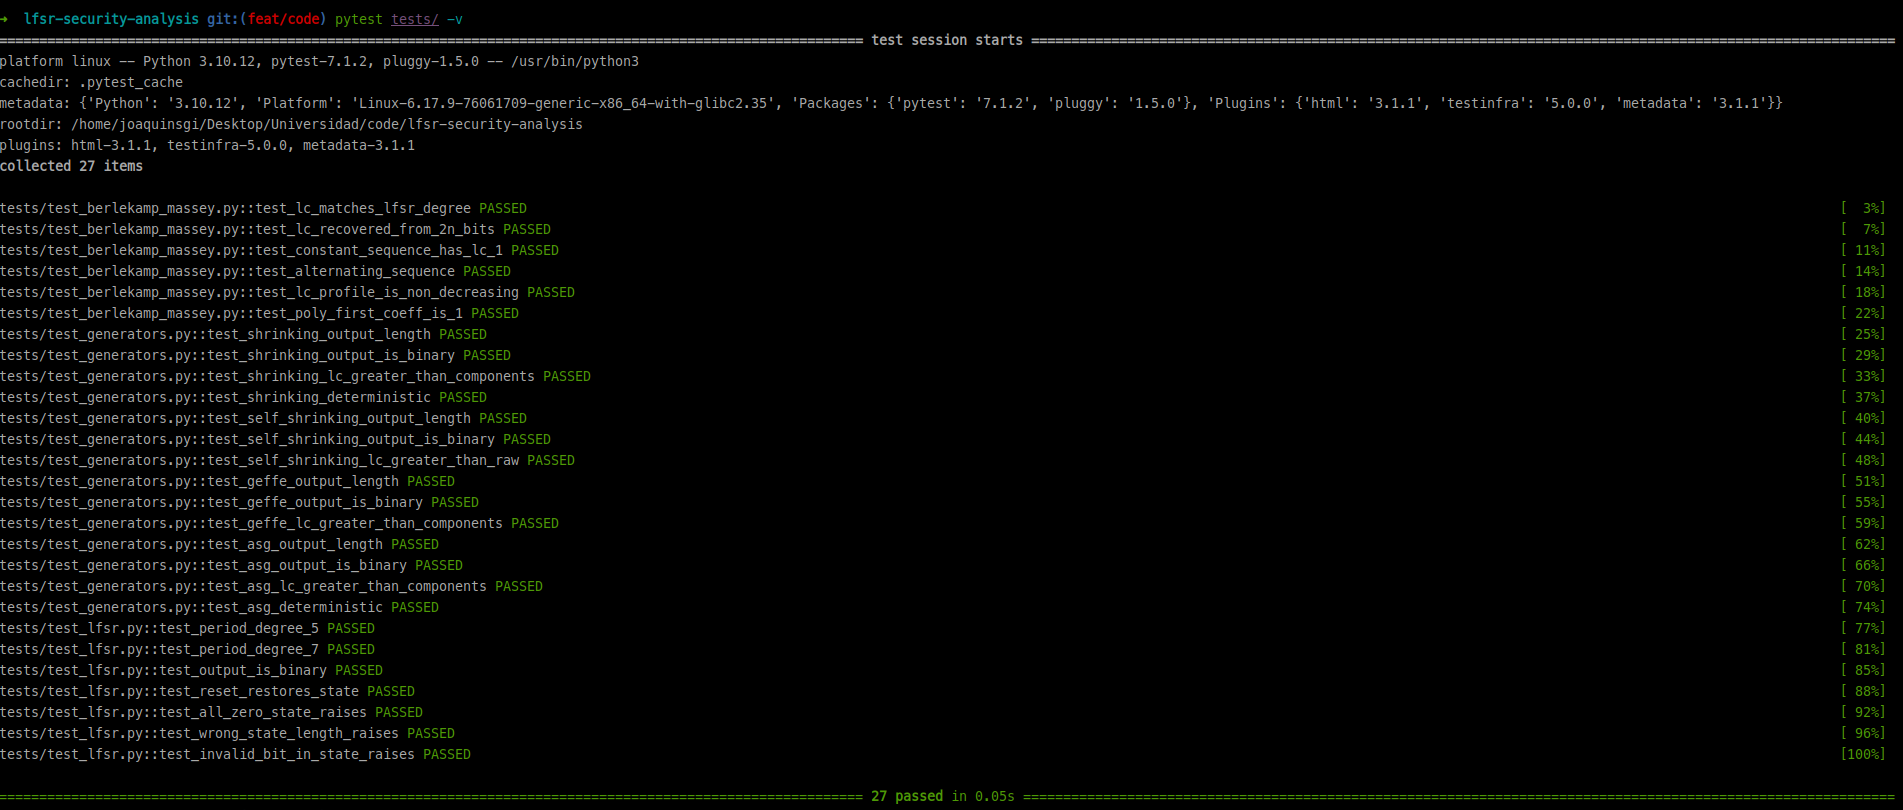
\includegraphics[width=0.9\textwidth]{images/execution_pytest.png}
\caption{Salida de \texttt{pytest tests/ -v}.}
\label{fig:exec-pytest}
\end{figure}

Esto no demuestra que la implementación sea correcta en sentido formal, ya que los tests cubren casos conocidos y no exhaustividad.
Pero sí da confianza razonable en que los p-valores de la tabla principal no son artefactos de un bug, sobre todo cuando los valores observados
coinciden cualitativamente con lo que predice la teoría (LFSR puro con LC igual al grado, Geffe con LC moderada, etc.).

Cuando uno de los resultados experimentales sorprendía (por ejemplo el p-valor de 0,012 del Self-Shrinking
en Block Frequency, ajustadísimo al umbral), poder ir al código del test y revisar paso a paso qué hacía el cálculo era exactamente lo que justifica
haber implementado todo desde cero en vez de tirar de librerías.

\section{Análisis por generador}

\subsection{LFSR puro}

Pasa 5 de 8 tests. Los tres que falla (Binary Matrix, Espectral y Complejidad lineal)
son precisamente los tres que detectan estructura lineal. Los cinco que pasa (Monobit, Block Frequency, Runs, Maurer y Serial)
evalúan propiedades estadísticas que las m-sequences cumplen de forma natural por las propiedades de Golomb.

Esto es importante, ya que si solo se mira con tests estadísticos básicos un LFSR puro \textit{parece} aceptable.
La diferencia entre apariencia y realidad se ve en su perfil de complejidad lineal, plano desde el bit 38 en adelante.
Y eso es exactamente lo que Berlekamp-Massey explota.

\subsection{Geffe}

Pasa 7 de 8 tests, con el espectral como único fallo. Estadísticamente se comporta bastante bien.
Pero recordemos del capítulo anterior, el problema real del generador de Geffe es la correlación $0{,}75$ con dos de los tres LFSR,
no la estadística de su salida. Un atacante no necesita aplicar Berlekamp-Massey,
puede romper cada registro por separado con coste $2^7 + 2^5 + 2^9 = 672$ operaciones para nuestros tamaños.

Lo curioso es que los tests NIST no detectan esa vulnerabilidad. Esto es importante, los tests evalúan calidad estadística,
no resistencia a ataques estructurales.

\subsection{Shrinking y Self-Shrinking}

Ambos generadores pasan 7 de 8 tests, fallando solo el espectral. Sus complejidades lineales son excelentes (2498 y 2501, prácticamente $N/2$).
Desde el punto de vista de Berlekamp-Massey son tan buenos como una secuencia aleatoria.

El fallo del espectral tiene una explicación intuitiva, la secuencia base sigue siendo la de un LFSR,
y aunque el muestreo irregular dispersa los picos espectrales del registro original,
no los elimina del todo. La DFT todavía detecta exceso de picos por encima del umbral teórico.

Es una debilidad teórica que no compromete la seguridad práctica (no se conocen ataques que exploten esta periodicidad residual),
pero es un detalle medible. En la práctica esto desaparece con LFSR de grado mayor, ya que los armónicos se diluyen en secuencias largas.

El Self-Shrinking además tiene el p-valor de block frequency más justo (0,012), muy cerca del umbral.
Esto sugiere que la selección irregular sobre la propia secuencia introduce algún desequilibrio local,
posiblemente porque selector y datos no son independientes.

\subsection{ASG}

Único que pasa los 8 tests con los parámetros usados. Su p-valor en el test espectral (0,825) no solo está por encima del umbral
sino que es alto incluso para una secuencia aleatoria. Eso indica que el mecanismo del ASG hace un trabajo particularmente bueno destruyendo periodicidades.

Lo más interesante es que el de ASG usa los mismos tres LFSR que el de Geffe. Mismo hardware, complejidad lineal 4x mayor y todos los tests pasados.
Reloj alterno con XOR de fuentes independientes funciona mucho mejor que un multiplexor de selección directa.

\section{Discusión}

\subsection{La complejidad lineal es necesaria pero no suficiente}

La tabla de resultados separa muy claramente a los generadores en dos grupos. En el primero, LFSR puro y Geffe,
con complejidad lineal baja (19 y 623). En el segundo, Shrinking, Self-Shrinking y ASG, con complejidad lineal cercana a $N/2$.

Sin embargo, dentro del segundo grupo la complejidad lineal sola no permite distinguir nada.
Los tres tienen valores prácticamente idénticos ($\sim 2500$) pero comportamiento muy distinto en el test espectral.
Tener complejidad lineal alta es condición necesaria (un generador con LC baja cae frente a Berlekamp-Massey) pero no garantiza calidad estadística completa.

\subsection{Los tests estadísticos no detectan todo}

El caso de Geffe es ilustrativo, pasa 7 de 8 tests pese a ser trivialmente atacable por correlación.
Los tests NIST detectan desviaciones estadísticas de la salida, pero no analizan la estructura interna del generador.
Para evaluar un generador hace falta combinar tests estadísticos, complejidad lineal y análisis de ataques específicos.

\subsection{El mecanismo de combinación es lo que importa}

La comparación Geffe vs ASG es la más reveladora del trabajo. Mismos LFSR, mismos polinomios, mismos estados iniciales.
La única diferencia es cómo se combinan, multiplexor vs reloj alterno con XOR.
El resultado, Geffe falla espectralmente y tiene correlación 0,75, ASG pasa todos los tests y no tiene correlación detectable.

Esta es probablemente la lección de diseño más clara del experimento.
En generadores basados en LFSR la clave no es el tamaño de los registros sino el mecanismo de combinación.

\section{Limitaciones del análisis}

Conviene tener presente lo que este análisis no cubre.

\textbf{Un solo estado inicial por generador.} Los resultados corresponden a una ejecución
con estados fijos. Para los p-valores cerca del umbral (como el 0,012 del Self-Shrinking en block frequency)
otro estado inicial podría dar resultados distintos. Un análisis más robusto repetiría con varios estados
y reportaría la distribución de p-valores.

\textbf{Tests no implementados.} Faltan 7 de los 15 tests del estándar.
Random excursions en particular podría detectar asimetrías que los implementados no cubren.

\textbf{Ataques no implementados.} El ataque de correlación contra Geffe se describe en teoría
pero no se ejecuta. Una extensión natural sería programarlo y verificar
que el coste real coincide con el predicho.

Pese a estas limitaciones, los resultados son coherentes con la teoría y permiten extraer conclusiones claras sobre la seguridad relativa de los cuatro generadores,
que es lo que se discute en el capítulo final.


\chapter{Conclusiones}
\label{cap:conclusiones}

\section{Resumen del trabajo}

Este trabajo ha consistido en implementar desde cero un entorno completo para el análisis de generadores pseudoaleatorios basados en LFSR
y usarlo para comparar cuatro construcciones clásicas, Geffe, Shrinking, Self-Shrinking y Alternating Step Generator.

El entorno incluye tres componentes principales. El primero es la implementación de los generadores, un LFSR genérico parametrizable por grado y polinomio,
y los cuatro generadores construidos sobre él. El segundo es el algoritmo de Berlekamp-Massey,
que permite medir la complejidad lineal de cualquier secuencia binaria y calcular su perfil de evolución.
El tercero son ocho tests del estándar NIST SP 800-22, cada uno evaluando un aspecto distinto de la aleatoriedad
(balance, distribución de rachas, rango matricial, compresibilidad, distribución de patrones, espectro de frecuencias y complejidad lineal por bloques).

Son unas 1500 líneas de Python escritas sin librerías criptográficas. Las únicas dependencias externas son scipy (funciones de distribución estadística),
numpy (operaciones con arrays) y matplotlib (gráficas). Hay 27 tests unitarios que verifican cada componente contra valores de referencia conocidos.

El análisis experimental se ha realizado con secuencias de 500.000 bits para los tests NIST y 5.000 bits para la complejidad lineal,
con un nivel de significación $\alpha = 0{,}01$. Los resultados principales son los siguientes,
el generador de ASG pasa los 8 tests con complejidad lineal cercana a $N/2$,
Shrinking y Self-Shrinking tienen complejidad lineal similar al ASG pero fallan el test espectral,
el generador de Geffe pasa 7 tests pero es vulnerable a ataques de correlación, y el LFSR puro falla los 3 tests que detectan estructura lineal.

\section{Conclusiones principales}

\subsection{La complejidad lineal es necesaria pero no suficiente}

La complejidad lineal separa claramente a los generadores en dos grupos. Por un lado el LFSR puro y Geffe,
con valores bajos respecto a la longitud de la secuencia. Por otro Shrinking, Self-Shrinking y ASG, con valores cercanos a $N/2$.
Sin embargo, dentro del segundo grupo la complejidad lineal no distingue la calidad real.

Geffe tiene complejidad lineal 623, mucho mayor que la del LFSR puro (19) pero baja en términos absolutos.
Aun así, su debilidad principal no es esa sino la correlación $0{,}75$ con dos de sus LFSR internos,
que permite un ataque con coste proporcional a la suma de los espacios de estados, no al producto.
Un atacante rompe Geffe mucho antes de lo que Berlekamp-Massey requeriría.

Los otros tres generadores tienen complejidades lineales casi idénticas ($\sim 2500$) pero comportamiento distinto en el test espectral,
y eso la complejidad lineal no lo captura. Tener LC alta es condición necesaria (un generador con LC baja cae frente a Berlekamp-Massey)
pero no basta para garantizar buenas propiedades estadísticas.

\subsection{Los tests estadísticos detectan propiedades, no seguridad}

Los tests NIST detectan desviaciones estadísticas en la secuencia de salida, no evalúan la seguridad del generador como construcción criptográfica.
Geffe pasa 7 de 8 tests pese a ser trivialmente atacable. El LFSR puro pasa 5 de 8 pese a ser completamente predecible con 38 bits observados.

Esto no significa que los tests sean inútiles. Si la salida tiene patrones detectables, el generador no puede ser seguro.
Pero pasar todos los tests no garantiza seguridad, solo que no hay defectos estadísticos evidentes.
Los tests filtran generadores con defectos obvios, no sustituyen al análisis de la estructura interna.

\subsection{El mecanismo de combinación determina la calidad}

De los cuatro generadores, el ASG es el que mejor se comporta tanto en complejidad lineal como en los tests estadísticos.
Pasa los 8 tests NIST con los mismos parámetros con los que los otros tres fallan al menos uno.
La diferencia está en su mecanismo de combinación, reloj irregular más XOR de dos fuentes independientes.

La comparación más clara es entre Geffe y ASG, ya que ambos usan exactamente los mismos tres LFSR.
La única diferencia es cómo se conectan. Geffe usa un multiplexor (selección directa con correlación) y ASG usa reloj alterno más XOR.
El resultado, Geffe tiene LC 623 y falla espectralmente, ASG tiene LC 2499 y pasa todo.
Mismo hardware, resultado completamente distinto.

La conclusión es clara, en generadores basados en LFSR la clave no es el tamaño de los registros sino cómo se combinan.
Un buen mecanismo convierte tres LFSR pequeños en un generador robusto, un mecanismo malo (el multiplexor de Geffe) deja el sistema vulnerable
da igual cuánto se agranden los registros.

\subsection{La selección irregular es buena pero no perfecta}

Shrinking y Self-Shrinking logran complejidades lineales excelentes y pasan 7 de 8 tests.
Su mecanismo de selección irregular destruye la estructura lineal de la secuencia base.
Sin embargo, ambos fallan el test espectral, lo que indica que la periodicidad del LFSR base no se elimina completamente con el muestreo.

Que el ASG (con un mecanismo distinto) sí pase el espectral sugiere que para eliminar las componentes frecuenciales
no basta con muestrear irregularmente una secuencia periódica, hace falta combinar dos fuentes independientes de forma que sus periodicidades
se cancelen mutuamente.

En la práctica esta debilidad espectral probablemente desaparece con LFSR de grado suficiente,
porque los armónicos se diluyen en secuencias largas. Pero con los grados pequeños usados en este experimento, la diferencia es medible.

\section{Cumplimiento de objetivos}

Se han cumplido todos los objetivos de la introducción.

\begin{enumerate}
  \item Se ha implementado un LFSR genérico y el algoritmo de Berlekamp-Massey desde cero en Python,
        con tests unitarios que verifican su corrección.
  \item Se han implementado los cuatro generadores (Geffe, Shrinking, Self-Shrinking y ASG),
        todos funcionales y verificados contra resultados conocidos.
  \item Se ha medido la complejidad lineal de cada generador,
        verificando que los valores experimentales son coherentes con las cotas teóricas.
  \item Se han pasado 8 tests NIST a las secuencias de cada generador con $\alpha = 0{,}01$,
        y se han comparado los resultados.
  \item Se han extraído conclusiones sobre la seguridad relativa de los generadores,
        justificadas tanto por los resultados experimentales como por la teoría.
\end{enumerate}

Además de estos objetivos explícitos, el trabajo ha producido un software completo y documentado que podría usarse como base para análisis más amplios
(con más tests, más generadores o parámetros más grandes).

\section{Trabajo futuro}

\subsection{Secuencias más largas y más estados iniciales}

El análisis usa un estado inicial fijo por generador. Una extensión natural es ejecutar los tests con múltiples estados iniciales seleccionados al azar
y reportar la distribución de p-valores en vez de un único valor.
Así se podría ver si los resultados cercanos al umbral (como el block frequency del Self-Shrinking con 0,012) son estables o dependen del estado concreto.

Otra dirección interesante es fijar la longitud de secuencia y variar los grados de los LFSR para trazar la frontera de detección,
a partir de qué grado mínimo el Shrinking empieza a pasar el test espectral.
El resultado sería una recomendación práctica de tamaño mínimo para cada generador.

\subsection{Implementación de ataques}

El ataque de correlación contra Geffe se ha descrito teóricamente pero no se ha implementado.
Una extensión interesante sería programarlo y verificar experimentalmente que el coste real coincide con el predicho ($2^{n_1} + 2^{n_2} + 2^{n_3}$).
Dado un fragmento de keystream observado, probar los $2^5 = 32$ estados posibles de $R_2$, generar la secuencia correspondiente y contar coincidencias.
El estado correcto debería dar coincidencia $\sim 75\%$ y uno incorrecto $\sim 50\%$.
Verificar esto en la práctica y medir cuántos bits necesita la distinción para ser fiable sería una demostración concreta de la vulnerabilidad.

También se podría implementar fuerza bruta sobre $R_1$ del Shrinking y medir cuántos bits son necesarios para identificar correctamente la secuencia de selección.

\subsection{Tests adicionales y herramientas externas}

Implementar los 7 tests NIST restantes daría una imagen más completa del comportamiento de cada generador.
Random excursions en particular podría revelar asimetrías que los implementados no detectan.

Para validar la implementación se podría ejecutar la batería NIST oficial (escrita en C por el propio NIST) sobre las mismas secuencias generadas por mi código.
Esto serviría como comprobación cruzada, y si los p-valores coinciden con la implementación oficial,
se tendría confianza adicional en la corrección.

\subsection{Generadores más recientes}

Los cuatro generadores estudiados son construcciones clásicas de los años 70-90.
Sería interesante repetir el análisis con generadores más recientes como Grain o Trivium (del proyecto eSTREAM),
que también están basados en registros de desplazamiento pero incorporan componentes no lineales más sofisticados.
Comparar estos con los clásicos permitiría ver cuánto ha avanzado el diseño de cifrados de flujo en las últimas décadas.

Grain combina un LFSR con un NLFSR (registro con retroalimentación no lineal) del mismo tamaño y aplica una función booleana de filtrado sobre ambos.
Implementar Grain con las mismas herramientas de este trabajo y compararlo con el ASG mostraría si el componente no lineal explícito da mejores resultados
que la no linealidad implícita del reloj irregular.

\section{Valoración personal}

Este trabajo me ha permitido entender la criptografía de flujo a un nivel de detalle que no habría conseguido solo leyendo sobre ella.
Implementar Berlekamp-Massey desde cero, por ejemplo, obliga a entender por qué funciona y cómo cada paso del algoritmo contribuye al resultado.
Lo mismo pasa con los tests NIST, ya que programar cada uno te fuerza a pensar en qué hipótesis estadística se está contrastando
y qué distribución teórica se asume.

La parte que me resultó más sorprendente fue que el ASG (con los mismos LFSR que el de Geffe) diera resultados tan superiores en los tests estadísticos.
Antes de hacer los experimentos esperaba que Shrinking y Self-Shrinking fueran los mejores por ser los más recientes.
Que el de ASG (de 1987, anterior a los otros dos) fuera el único en pasar todos los tests fue contraintuitivo hasta entender la razón,
el XOR con reloj alterno destruye la periodicidad de una forma que el muestreo irregular no consigue.

También me pareció instructivo ver que el LFSR puro pasa 5 de 8 tests. Si solo se evaluara con tests estadísticos básicos parecería un generador aceptable.
Esto refuerza algo que leí varias veces pero no terminaba de interiorizar, las propiedades estadísticas y la seguridad criptográfica son cosas distintas.
Para evaluar un generador hay que atacarlo, no solo testearlo.

Me llevo el haber aprendido a usar un asistente de inteligencia artificial como apoyo para revisar el código y la redacción.
Esto vino a raiz de que en mi plano profesional nos animaban a usar estas herramientas de manera constructiva, ya que se observaba una gran mejora en la calidad del trabajo cuando se usaban correctamente,
ademas, de un claro beneficio en el tiempo de trabajo, ya que uno empieza a usarlas como un colaborador que revisa tu trabajo, y lo emplea para contrastar, encontrar erratas o cuestionar una explicación poco clara, revisando siempre lo que devuelve.
Es una herramienta que en el entorno laboral se pide cada vez más, y saber usarla de forma crítica (sin delegar en ella el criterio) me parece una competencia tan valiosa como las
puramente técnicas del trabajo.

Por último, la decisión de implementar todo desde cero ha sido la que más tiempo ha costado pero también la que más me ha enseñado.
Programar el test espectral, por ejemplo, me obligó a entender la DFT a un nivel que de otra forma no habría necesitado.
Y cuando el Self-Shrinking dio un p-valor de 0,012 en block frequency, pude ir directamente al código del test a comprobar que no era un bug
(no lo era, simplemente esa secuencia concreta tiene un bloque con desequilibrio local). Esa capacidad de ir al código y entender exactamente qué pasa
es lo que justifica el esfuerzo de no usar librerías externas.


\appendix
\chapter{Instalación y uso del repositorio}
\label{ap:instalacion}

Todo el código que se ha utilizado en este trabajo está disponible en un repositorio público de Git.
El objetivo de este apéndice es dar las indicaciones mínimas para que cualquier lector pueda clonar el repositorio,
instalar las dependencias y reproducir los experimentos sobre los que se construye el capítulo~\ref{cap:analisis}.

\section{Estructura del repositorio}

El repositorio se organiza con dos ramas separadas. La rama \texttt{feat/code} contiene el código fuente,
los tests unitarios y los resultados (la rama \texttt{feat/docs} contiene la memoria en \LaTeX{}, que es la que se está leyendo).
La separación entre ambas permite trabajar de forma independiente en el código y en la memoria
sin que un cambio en una parte afecte al historial de la otra.

Dentro de \texttt{feat/code}, el árbol de directorios es el siguiente.

\begin{lstlisting}[basicstyle=\small\ttfamily,frame=single,backgroundcolor=\color{gray97},numbers=none]
src/
  lfsr.py                  # LFSR generico
  berlekamp_massey.py      # algoritmo de Berlekamp-Massey
  tests_nist/              # ocho tests del estandar NIST SP 800-22
    monobit.py
    block_frequency.py
    runs.py
    binary_matrix.py
    maurer.py
    serial.py
    spectral.py
    linear_complexity.py
  generators/              # generadores basados en LFSR
    geffe.py
    shrinking.py
    self_shrinking.py
    alternating_step.py
  analysis/
    run_experiments.py     # script principal de experimentos
    plots.py               # generacion de figuras

tests/                     # tests unitarios (pytest)
results/                   # resultados generados (JSON + PNGs)
requirements.txt           # dependencias Python
\end{lstlisting}

\section{Requisitos}

El código está escrito en Python~3.10 o superior y depende de tres librerías externas.
\texttt{numpy} se usa para las operaciones sobre arrays de bits y para la FFT del test espectral,
\texttt{scipy} aporta las funciones especiales (gamma incompleta y función de error complementaria)
que necesitan varios tests estadísticos, y \texttt{matplotlib} se utiliza para generar las gráficas de complejidad lineal
y de comparación entre generadores. \texttt{pytest} se usa solo para ejecutar los tests unitarios.

Las versiones mínimas están fijadas en \texttt{requirements.txt}.

\begin{lstlisting}[basicstyle=\small\ttfamily,frame=single,backgroundcolor=\color{gray97},numbers=none]
numpy>=1.24
scipy>=1.10
matplotlib>=3.7
pytest>=7.0
\end{lstlisting}

\section{Instalación}

Los pasos para clonar el repositorio e instalar las dependencias son los habituales en cualquier proyecto Python.
Conviene crear un entorno virtual para que las versiones de las librerías no entren en conflicto con otros proyectos del sistema.

\begin{lstlisting}[style=Terminal]
$ git clone https://github.com/joaquinsgi/lfsr-security-analysis.git
$ cd lfsr-security-analysis
$ git checkout feat/code
$ python -m venv venv
$ source venv/bin/activate
(venv) $ pip install -r requirements.txt
\end{lstlisting}

Una vez instaladas las dependencias, el repositorio queda listo para ejecutar tanto los tests unitarios
como los experimentos completos.

\section{Ejecución de los tests unitarios}

El proyecto incluye 27 tests unitarios distribuidos en tres ficheros, uno para el LFSR, uno para Berlekamp-Massey y uno para los cuatro generadores.
Sirven para garantizar que las funcionalidades básicas son correctas y que un cambio futuro no rompe lo ya implementado.
Se ejecutan con \texttt{pytest} desde la raíz del repositorio.

\begin{figure}[H]
\centering
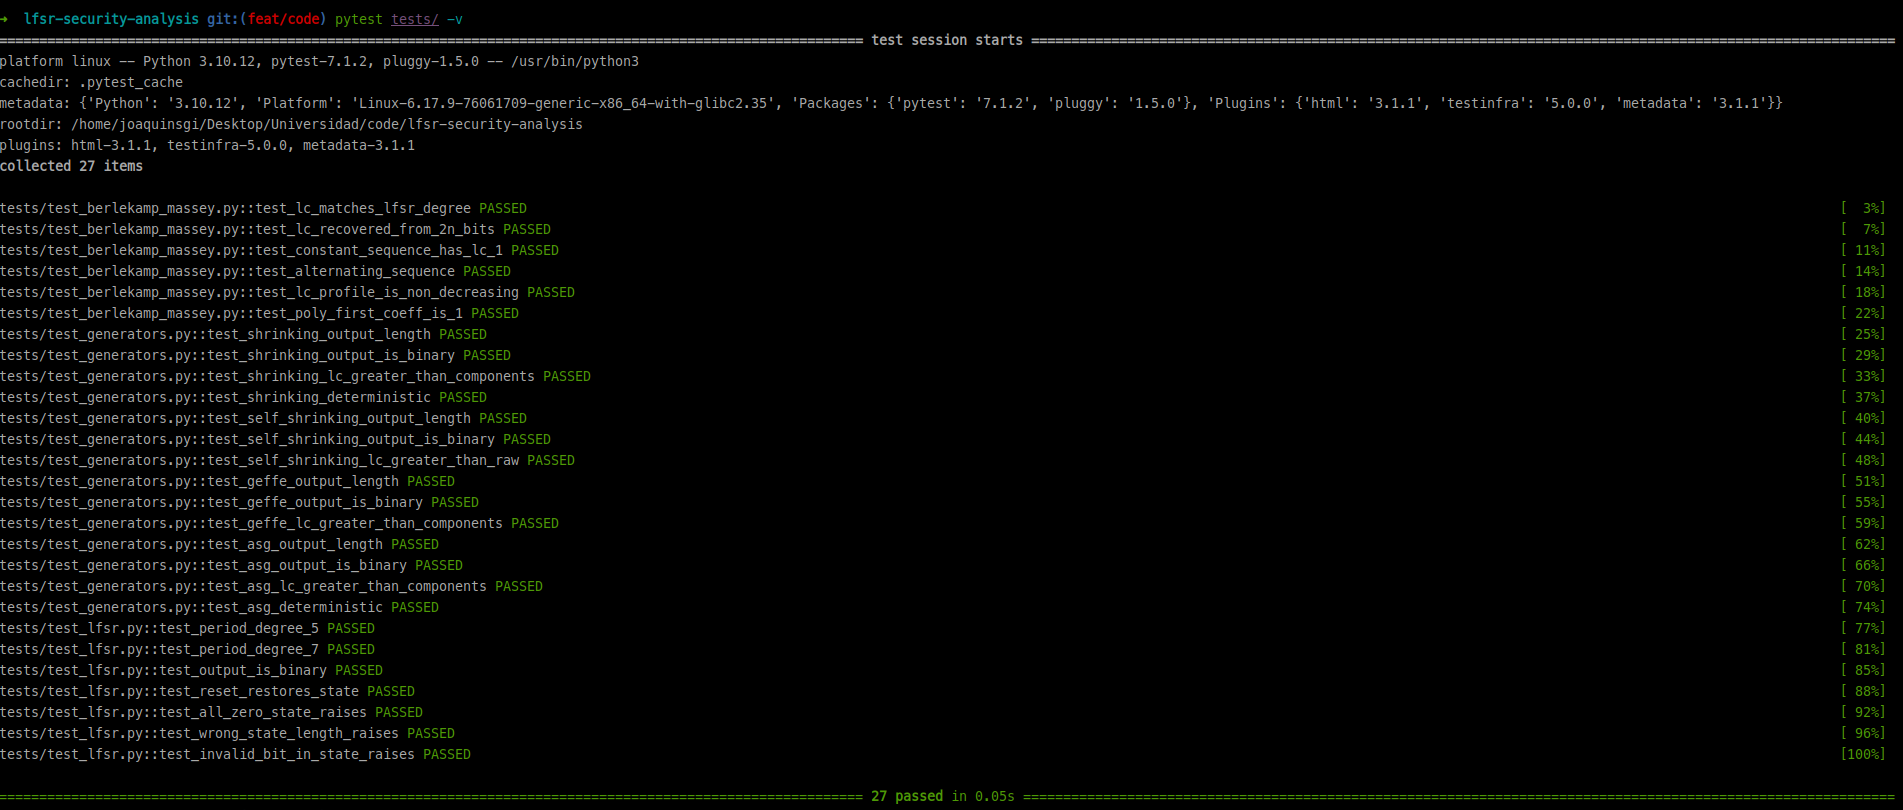
\includegraphics[width=0.9\textwidth]{images/execution_pytest.png}
\caption{Salida de \texttt{pytest tests/ -v} sobre el árbol completo.}
\label{fig:exec-pytest-appendix}
\end{figure}

Que los 27 tests pasen no garantiza que el análisis del capítulo~\ref{cap:analisis} sea correcto,
ya que los tests cubren la lógica interna pero no el experimento al completo.
Sí garantiza que cada componente aislado se comporta como se espera,
y por tanto cualquier discrepancia en los resultados experimentales no es atribuible a errores básicos de implementación.

\section{Ejecución del experimento principal}

El script \texttt{run\_experiments.py} reproduce el flujo completo del capítulo~\ref{cap:analisis}.
Genera secuencias de 500.000 bits con los cuatro generadores, calcula la complejidad lineal de los primeros 5.000 bits
con Berlekamp-Massey, aplica los ocho tests NIST a cada secuencia y serializa los resultados en \texttt{results/results.json}.

\begin{figure}[H]
\centering
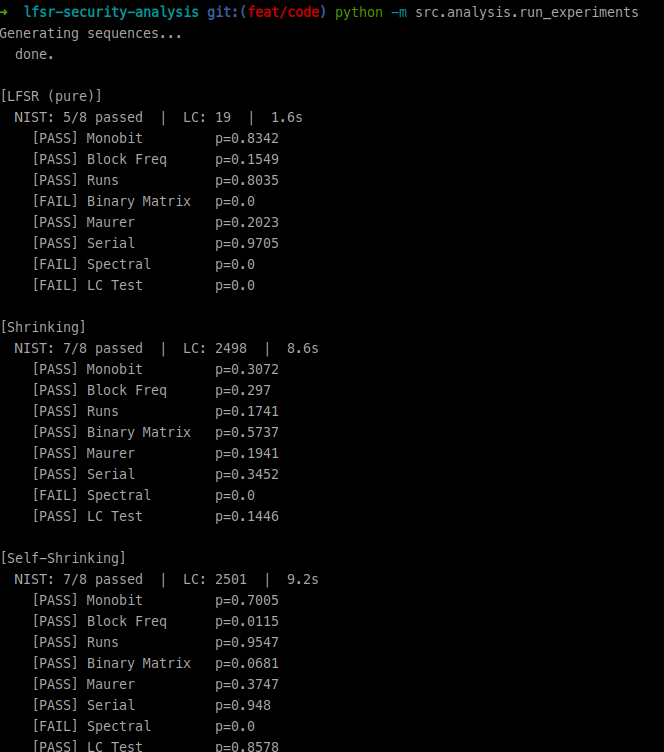
\includegraphics[width=0.9\textwidth]{images/execution_run_experiments_1.png}
\caption{Salida de \texttt{python -m src.analysis.run\_experiments} (parte 1).}
\label{fig:exec-run-experiments-app-1}
\end{figure}

\begin{figure}[H]
\centering
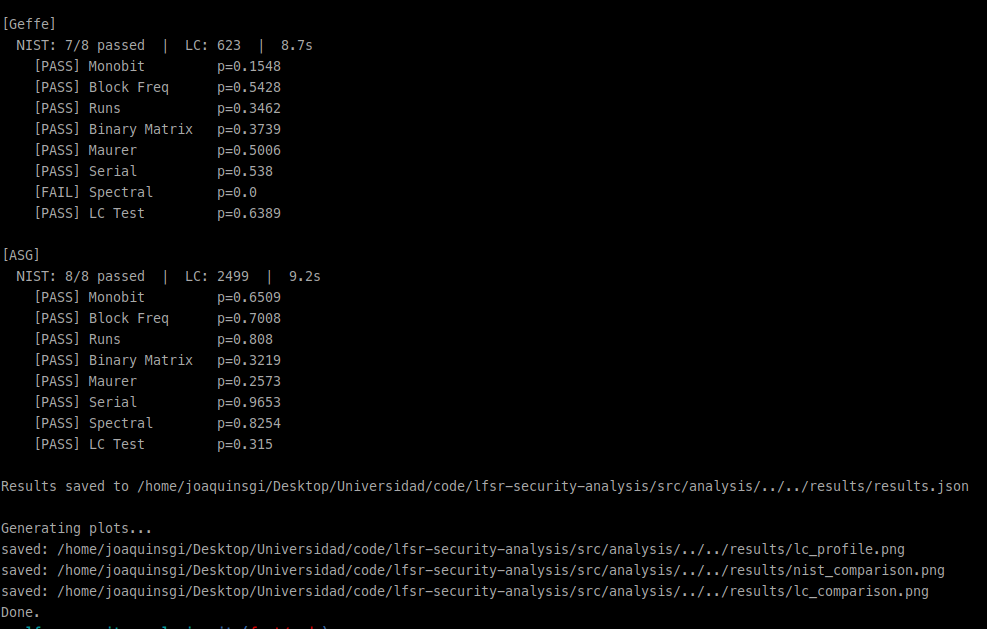
\includegraphics[width=0.9\textwidth]{images/execution_run_experiments_2.png}
\caption{Salida de \texttt{python -m src.analysis.run\_experiments} (parte 2).}
\label{fig:exec-run-experiments-app-2}
\end{figure}

Como parte de la misma ejecución, \texttt{run\_experiments.py} regenera las tres gráficas de complejidad lineal
y comparación entre generadores que aparecen en el capítulo~\ref{cap:analisis} (\texttt{results/lc\_profile.png},
\texttt{results/lc\_comparison.png} y \texttt{results/nist\_comparison.png}).

Con esto cualquier lector puede repetir el experimento completo y comparar sus resultados con los que aparecen en la memoria.
Las pequeñas variaciones en los p-valores son normales si se cambian los estados iniciales de los LFSR,
pero el comportamiento global (qué generadores pasan qué tests, qué generador obtiene complejidad lineal alta)
se mantiene estable y coincide con el análisis del capítulo~\ref{cap:analisis}.


\nocite{*}
\bibliography{bibliography/bibliography}\addcontentsline{toc}{chapter}{Bibliografía}
\bibliographystyle{plain}

\end{document}
